\documentclass[12pt]{article}
\usepackage{fullpage}
\usepackage{combelow}
\usepackage{amsmath,amssymb,amsthm}
\usepackage{graphicx}
\usepackage{tikz}
\usepackage{booktabs}
\usepackage{array}
\usepackage[shortlabels]{enumitem}
\usepackage{needspace}
\setlength{\emergencystretch}{2em}
\usepackage[colorlinks=true,linkcolor=blue!45!black,citecolor=blue!45!black,urlcolor=blue!45!black]{hyperref}
\hypersetup{pdftitle={Maximum Blackouts That Keep Every Lattice Rectangle Identifiable},pdfauthor={Arjun Pemmasani}}

\definecolor{kgray}{HTML}{AAAAAA}
\definecolor{kyellow}{HTML}{FFF64C}
\definecolor{kred}{HTML}{FF6666}
\definecolor{kblue}{HTML}{4A86E8}
\tikzset{
  lab/.style={font=\scriptsize,text=black!55},
  capt/.style={font=\small},
}

\theoremstyle{plain}
\newtheorem{theorem}{Theorem}
\newtheorem{lemma}[theorem]{Lemma}
\newtheorem{proposition}[theorem]{Proposition}
\newtheorem{corollary}[theorem]{Corollary}
\newtheorem{introthm}{Theorem}
\renewcommand{\theintrothm}{\Alph{introthm}}
\theoremstyle{definition}
\newtheorem{definition}[theorem]{Definition}
\theoremstyle{remark}
\newtheorem{remark}[theorem]{Remark}

\newcommand{\seqnum}[1]{\href{https://oeis.org/#1}{\rm \underline{#1}}}
\newcommand{\pres}{P_S}
\newcommand{\kA}{\mathsf{A}}
\newcommand{\kB}{\mathsf{B}}
\newcommand{\kC}{\mathsf{C}}
\newcommand{\kE}{\mathsf{E}}

\title{Maximum Blackouts That Keep Every Lattice Rectangle Identifiable}
\author{Arjun Pemmasani\\
Department of Mathematics\\
Harvey Mudd College\\
Claremont, CA 91711\\
USA\\
\texttt{apemmasani@hmc.edu}}
\date{}

\begin{document}
\maketitle

\begin{abstract}
How many points of a grid can we black out while every rectangle, tilted or not,
remains determined by its white corners? This is Kagey's Problem 001. A row-column
graph and Mantel's theorem bound the maximum by the width plus the integer part
of a quarter of the squared height. We attain this bound at every height for all
sufficiently large widths by spacing columns with two black points between runs
black in alternating boundary rows. We determine
the maximum on up to six rows at every width, and on seven rows from width 24 on.
The five-row result refutes our earlier guess that the maximum is the sum of the
sides. We count the three-row optima exactly and find the growth rate on four rows.
At fixed height, the maximum minus the width is eventually periodic, and the
optimum counts have a rational generating function. The maxima and counts are
tabulated in A397315 and A399580 of the On-Line Encyclopedia of Integer Sequences.
Some values require computer checks.
\end{abstract}

\section{Introduction}\label{sec:intro}

Start with an $h\times m$ grid and black out some of its points.
The game master chooses a rectangle (tilted ones are allowed) and tells
you which of its corners are white. Can you recover all four corners?
Kagey~\cite{kageyG4G14,kagey001} asks how many points can be blacked out
while keeping the answer unique for every rectangle.
Such a set is a \emph{valid blackout} (Definition~\ref{def:valid}).
One round is shown in Figure~\ref{fig:game}.

\begin{figure}[t]
\centering
\resizebox{\textwidth}{!}{\begin{tikzpicture}[x=0.630cm,y=0.630cm,baseline=(current bounding box.north)]
  \draw[gridcol] (1,-1) grid (4,-3);
  \filldraw[fill=white,draw=keptline,line width=0.6pt] (1,-1) circle (0.17);
  \filldraw[fill=white,draw=keptline,line width=0.6pt] (2,-1) circle (0.17);
  \filldraw[fill=white,draw=keptline,line width=0.6pt] (3,-1) circle (0.17);
  \filldraw[fill=white,draw=keptline,line width=0.6pt] (4,-1) circle (0.17);
  \filldraw[fill=white,draw=keptline,line width=0.6pt] (1,-2) circle (0.17);
  \filldraw[fill=white,draw=keptline,line width=0.6pt] (2,-2) circle (0.17);
  \filldraw[fill=white,draw=keptline,line width=0.6pt] (3,-2) circle (0.17);
  \filldraw[fill=white,draw=keptline,line width=0.6pt] (4,-2) circle (0.17);
  \filldraw[fill=white,draw=keptline,line width=0.6pt] (1,-3) circle (0.17);
  \filldraw[fill=white,draw=keptline,line width=0.6pt] (2,-3) circle (0.17);
  \filldraw[fill=white,draw=keptline,line width=0.6pt] (3,-3) circle (0.17);
  \filldraw[fill=white,draw=keptline,line width=0.6pt] (4,-3) circle (0.17);
  \node[lab] at (1,-0.35) {1};
  \node[lab] at (2,-0.35) {2};
  \node[lab] at (3,-0.35) {3};
  \node[lab] at (4,-0.35) {4};
  \node[lab] at (0.35,-1) {1};
  \node[lab] at (0.35,-2) {2};
  \node[lab] at (0.35,-3) {3};
  \draw[rectB,line width=1.1pt] (3,-2) circle (0.3);
  \node[capt,anchor=north,text width=3.28cm,align=center] at (2.5,-3.7) {(a) the point $(3,2)$ is ringed};
  \draw[gridcol] (6.6,-1) grid (9.6,-3);
  \fill[black] (6.6,-1) circle (0.17);
  \fill[black] (7.6,-1) circle (0.17);
  \fill[black] (8.6,-1) circle (0.17);
  \fill[black] (9.6,-1) circle (0.17);
  \fill[black] (6.6,-2) circle (0.17);
  \filldraw[fill=white,draw=keptline,line width=0.6pt] (7.6,-2) circle (0.17);
  \filldraw[fill=white,draw=keptline,line width=0.6pt] (8.6,-2) circle (0.17);
  \filldraw[fill=white,draw=keptline,line width=0.6pt] (9.6,-2) circle (0.17);
  \fill[black] (6.6,-3) circle (0.17);
  \filldraw[fill=white,draw=keptline,line width=0.6pt] (7.6,-3) circle (0.17);
  \filldraw[fill=white,draw=keptline,line width=0.6pt] (8.6,-3) circle (0.17);
  \filldraw[fill=white,draw=keptline,line width=0.6pt] (9.6,-3) circle (0.17);
  \node[lab] at (6.6,-0.35) {1};
  \node[lab] at (7.6,-0.35) {2};
  \node[lab] at (8.6,-0.35) {3};
  \node[lab] at (9.6,-0.35) {4};
  \node[lab] at (5.949999999999999,-1) {1};
  \node[lab] at (5.949999999999999,-2) {2};
  \node[lab] at (5.949999999999999,-3) {3};
  \node[capt,anchor=north,text width=3.28cm,align=center] at (8.1,-3.7) {(b) our blackout};
  \draw[gridcol] (12.2,-1) grid (15.2,-3);
  \fill[black] (12.2,-1) circle (0.17);
  \fill[black] (13.2,-1) circle (0.17);
  \fill[black] (14.2,-1) circle (0.17);
  \fill[black] (15.2,-1) circle (0.17);
  \fill[black] (12.2,-2) circle (0.17);
  \filldraw[fill=white,draw=keptline,line width=0.6pt] (13.2,-2) circle (0.17);
  \filldraw[fill=white,draw=keptline,line width=0.6pt] (14.2,-2) circle (0.17);
  \filldraw[fill=white,draw=keptline,line width=0.6pt] (15.2,-2) circle (0.17);
  \fill[black] (12.2,-3) circle (0.17);
  \filldraw[fill=white,draw=keptline,line width=0.6pt] (13.2,-3) circle (0.17);
  \filldraw[fill=white,draw=keptline,line width=0.6pt] (14.2,-3) circle (0.17);
  \filldraw[fill=white,draw=keptline,line width=0.6pt] (15.2,-3) circle (0.17);
  \node[lab] at (12.2,-0.35) {1};
  \node[lab] at (13.2,-0.35) {2};
  \node[lab] at (14.2,-0.35) {3};
  \node[lab] at (15.2,-0.35) {4};
  \node[lab] at (11.549999999999999,-1) {1};
  \node[lab] at (11.549999999999999,-2) {2};
  \node[lab] at (11.549999999999999,-3) {3};
  \draw[draw=rectA,line width=1.6pt,line join=round,dash pattern=on 3pt off 2pt] (14.2,-1) -- (15.2,-2) -- (14.2,-3) -- (13.2,-2) -- cycle;
  \node[capt,anchor=north,text width=3.28cm,align=center] at (13.7,-3.7) {(c) the rectangle};
  \draw[gridcol] (17.799999999999997,-1) grid (20.799999999999997,-3);
  \draw[hidcol,line width=0.5pt] (17.799999999999997,-1) circle (0.09350000000000001);
  \draw[hidcol,line width=0.5pt] (18.799999999999997,-1) circle (0.09350000000000001);
  \draw[hidcol,line width=0.5pt] (19.799999999999997,-1) circle (0.09350000000000001);
  \draw[hidcol,line width=0.5pt] (20.799999999999997,-1) circle (0.09350000000000001);
  \draw[hidcol,line width=0.5pt] (17.799999999999997,-2) circle (0.09350000000000001);
  \filldraw[fill=white,draw=keptline,line width=0.6pt] (18.799999999999997,-2) circle (0.17);
  \draw[hidcol,line width=0.5pt] (19.799999999999997,-2) circle (0.09350000000000001);
  \filldraw[fill=white,draw=keptline,line width=0.6pt] (20.799999999999997,-2) circle (0.17);
  \draw[hidcol,line width=0.5pt] (17.799999999999997,-3) circle (0.09350000000000001);
  \draw[hidcol,line width=0.5pt] (18.799999999999997,-3) circle (0.09350000000000001);
  \filldraw[fill=white,draw=keptline,line width=0.6pt] (19.799999999999997,-3) circle (0.17);
  \draw[hidcol,line width=0.5pt] (20.799999999999997,-3) circle (0.09350000000000001);
  \node[lab] at (17.799999999999997,-0.35) {1};
  \node[lab] at (18.799999999999997,-0.35) {2};
  \node[lab] at (19.799999999999997,-0.35) {3};
  \node[lab] at (20.799999999999997,-0.35) {4};
  \node[lab] at (17.15,-1) {1};
  \node[lab] at (17.15,-2) {2};
  \node[lab] at (17.15,-3) {3};
  \draw[rectA,line width=1.1pt] (18.799999999999997,-2) circle (0.3);
  \draw[rectA,line width=1.1pt] (20.799999999999997,-2) circle (0.3);
  \draw[rectA,line width=1.1pt] (19.799999999999997,-3) circle (0.3);
  \node[capt,anchor=north,text width=3.28cm,align=center] at (19.299999999999997,-3.7) {(d) what we are shown};
\end{tikzpicture}
}
\caption{One round on a largest valid blackout of the $3\times4$ grid
(Section~\ref{sec:three}). Points are (column, row). Gray crossed circles are black. Panel (c) shows the red
rectangle, and (d) its yellow corners. The three yellow corners fix the fourth by
Lemma~\ref{lem:threecorners}.}
\label{fig:game}
\end{figure}

Write $f(h,m)$ for the most points we can black out, and $a_h(m)$
for the number of ways to attain it. The conjectures recorded in the
OEIS entry \seqnum{A397315}~\cite{oeis} were
$f(3,m)=m+2$ and $f(h,m)=h+m$ for $\min(h,m)\ge4$, with exceptions
$f(4,4)=7$ and $f(4,5)=8$. The first was proved in Lean by the Omega
Institute, whose pull request was merged on 15 September
2026~\cite{trureturing2026}. Our independent proof combines the row
bound (Theorem~\ref{thm:rowbound}) and the boundary cross
(Lemma~\ref{lem:cross}). The second guess breaks at $5\times8$
(Theorem~\ref{thm:fiverow}). Throughout, put $q_h=\lfloor h^2/4\rfloor$.
Computer-assisted claims are marked, and the supplement to this paper lists the
evidence for each.
% TODO(author): add the date of A397315 after its A-number (item S6).

The main results follow, with proof locations in parentheses.

\begin{introthm}[narrow grids]\label{thm:A}
\leavevmode
\begin{enumerate}[(a)]
\item We have $f(h,m)\ge h+m-1$, and $f(h,m)\le m+q_h$ if $m\ge3$. \textup{(Lemma~\ref{lem:cross}
and Theorem~\ref{thm:rowbound}, Section~\ref{sec:graph}.)}
\item We have $f(2,m)=m+1$ and $f(3,m)=m+2$ for $m\ge3$, $f(4,m)=m+4$ for $m\ge6$,
and $f(5,5)=10$. \textup{(Theorem~\ref{thm:strip}, Section~\ref{sec:three},
Theorem~\ref{thm:fourvalue}, and Theorem~\ref{thm:fivefive}(a).)}
\item (Computer-assisted, with checked certificates for $f(5,6)$ and $f(5,7)$, and the last
claim checked in Lean.) We have $f(4,4)=7$, $f(4,5)=8$,
$f(5,6)=11$, $f(5,7)=12$, and $f(5,m)=m+6$ for $m\ge8$. \textup{(Corollary~\ref{cor:fourboundary}
and Theorem~\ref{thm:fiverow}(a), (b).)}
\item (Computer-assisted for $m\le14$, with checked certificates for the upper bounds, and
checked in Lean for $m\ge15$.) We have $f(6,m)=m+7$ for $8\le m\le11$, $f(6,m)=m+8$ for
$12\le m\le14$, and $f(6,m)=m+9$ for $m\ge15$. \textup{(Theorem~\ref{thm:sixrow}.)}
\item (Computer-assisted, with checked certificates.) We have $f(6,6)=12$,
$f(6,7)=13$, $f(7,7)=14$, and $f(6,8)=15$. \textup{(Theorem~\ref{thm:refute}.)}
\item (Computer-assisted.) We have $f(7,m)=m+12$ for every $m\ge24$.
\textup{(Theorem~\ref{thm:sevenrow}.)}
\end{enumerate}
\end{introthm}

With (e) and transposition, $f(h,m)$ is known for every $h\le6$ and every $m$.
For (c) and (d), the collar theorem reduces each infinite family to
one validity check (Theorem~\ref{thm:collar}). Lemma~\ref{lem:enc}
justifies the SAT bounds.

\begin{introthm}[three-row optima]\label{thm:B}
\leavevmode
\begin{enumerate}[(a)]
\item For $m\ge4$ the counts $a_3(m)$ \textup{(}\seqnum{A401223}\textup{)} satisfy $a_3(m)=4(m-1)(3m+2)\,3^{m-5}+E_m$, where $E_m>0$ counts the
optima with a column black in rows $1$ and $3$ (\seqnum{A398448}), and
$E_m=O(m^2(1+\sqrt3)^m)$. So $a_3(m)\sim\frac4{81}m^23^m$, and a fraction tending to $4/27$
of the $m^23^{m-1}$ axis-valid candidates is valid. The series $\sum_{m\ge3}a_3(m)z^m$ is
rational, and its denominator divides $(1-3z)^3(1-2z-2z^2)^3(1+2z^2)^3$.
\textup{(Theorem~\ref{thm:threecount}, Proposition~\ref{prop:threeclass}(c), the last claims of
Theorem~\ref{thm:threeclosed}, and Theorem~\ref{thm:threegf}(a), Section~\ref{sec:three}.)}
\item (Computer-assisted, exact computer algebra.) This is the reduced denominator,
and $E_m\sim\frac{19+11\sqrt3}{432}m^2(1+\sqrt3)^m$. \textup{(Theorem~\ref{thm:threegf}(b),
proved in Section~\ref{app:threegf}, and Theorem~\ref{thm:threeclosed}.)}
\end{enumerate}
\end{introthm}

\begin{introthm}[four rows]\label{thm:C}
If $m\ge4$, no valid blackout of the $4\times m$ grid hides all corners of a
rectangle \textup{(Theorem~\ref{thm:hidden})}. (Computer-assisted.) The series
$\sum_{m\ge6}a_4(m)z^m$ of the counts in \seqnum{A401224} is rational with reduced denominator of degree $420$, and
$a_4(m)\sim c\,m^4\rho_4^m$ with $c\approx8.1611\times10^{-5}$ and $\rho_4=3.35199\ldots$, an
algebraic number of degree $20$ \textup{(Proposition~\ref{prop:fourautomaton},
Theorem~\ref{thm:fourgfexact}, and Corollary~\ref{cor:fourgrowth}, Section~\ref{sec:four})}.
\end{introthm}

\begin{introthm}[every height at large widths]\label{thm:D}
For every $h\ge3$ we have $f(h,m)=m+q_h$ once $m\ge q_h+(q_h-1)(2W_h+1)$, where
$W_h=1+\lfloor(h-1)^2/4\rfloor$. \textup{(Theorem~\ref{thm:general},
Section~\ref{sec:general}.)}
\end{introthm}

\begin{introthm}[every fixed height]\label{thm:E}
Fix $h\ge1$ and write a blackout as the word $B_1\cdots B_m$ of the black rows of its
columns. The valid words form a regular language. If $h\ge2$, then $f(h,m)-m$ is
eventually periodic in $m$, and $\sum_{m\ge0}a_h(m)z^m$ is rational.
\textup{(Theorems~\ref{thm:regular} and~\ref{thm:periodic}, Section~\ref{sec:height}.)}
\end{introthm}

Corollary~\ref{cor:oeisconj} proves the conjecture in \seqnum{A338885} that its row $n$ has
largest entry \seqnum{A033638}$(n)$.

\paragraph{Prior work.} Choosing white points to distinguish rectangles is
a test-cover problem~\cite{bellitto2018,foucaud2015,katona1966,moretshapiro1985}
(Corollary~\ref{cor:hitting}). If we only forbid fully black axis-aligned
rectangles, we get the Zarankiewicz problem~\cite{furedi1996,kst1954,reiman1958}.
To distinguish all axis-aligned rectangles, the row-column graph must
avoid both four- and six-cycles (Lemma~\ref{lem:girth}). Such graphs,
including unbalanced parts, are studied by de Caen and
Sz\'ekely~\cite{decaenszekely1992,decaenszekely1997}. With $n$ vertices on each
side, the largest ones have $\Theta(n^{4/3})$ edges. Incidence graphs of generalized
quadrangles attain this order~\cite{benson1966}, and Hoory~\cite{hoory2002} and
Neuwirth~\cite{neuwirth2001} bound it from above. Lazebnik, Ustimenko, and
Woldar~\cite{lazebnik1995} construct dense graphs of every even girth.
Neuwirth's edge bounds~\cite[Theorem~1(ii) and Proposition~17]{neuwirth2001}
already give our row bound in graph form. Our Mantel proof~\cite{mantel1907} also classifies and counts
the equality cases.
The tilted rectangles require additional arguments.
For fixed height, our column method uses transfer
matrices~\cite{alanko2011,euler2005,mertens2024},
\cite[Proposition~V.6]{flajolet2009}.
Theorem~1(3) of Guilhot, Little, and Parkinson~\cite{glp2025} also
yields Theorem~\ref{thm:E} once regularity is proved.

\paragraph{Outline.} Sections~\ref{sec:conv} to~\ref{sec:graph} set up
the problem and its graph bounds. Sections~\ref{sec:three}
to~\ref{sec:five} handle narrow grids, Section~\ref{sec:general} every height at large
widths, and Section~\ref{sec:height} fixed height.
Section~\ref{sec:square} gives the square-grid bounds,
Section~\ref{sec:verify} the computational evidence and encoding
proofs, and Section~\ref{sec:open} the open questions.

\section{Conventions}\label{sec:conv}

We record the black points column by column, using the following notation.

\begin{enumerate}[(1),leftmargin=*]
\item An $h\times m$ grid has $h$ rows, $m$ columns, and point set $V$. A $2\times m$ grid
is a \emph{strip}. The point $(i,j)$ lies in column $i$ and row $j$, with $(1,1)$ at the
top left (Figure~\ref{fig:game}(a)).
\item A \emph{rectangle} has four grid points as corners and positive area.
We write $C(R)$ for its corner set. It is \emph{axis-aligned} if its sides
follow the grid lines, and \emph{tilted} otherwise.
\item A \emph{blackout} is the set $S\subseteq V$ of black points. Its
\emph{kept set} is $K=V\setminus S$, and the \emph{presentation}
$\pres(R)=C(R)\setminus S$ is what the rectangle shows, namely its white corners.
\item Column $i$ has \emph{black rows} $B_i=\{j:(i,j)\in S\}$, and is \emph{empty}, a
\emph{singleton}, a \emph{double}, or a \emph{triple} when $|B_i|$ is $0$, $1$, $2$, or
$3$, and \emph{full} when $|B_i|=h$. The \emph{pair set} $F$ is the set of row pairs
contained in some $B_i$, and $q_h=\lfloor h^2/4\rfloor$ is \seqnum{A002620}$(h)$.
\end{enumerate}

\begin{definition}[valid blackout]\label{def:valid}
A blackout $S$ is \emph{valid} if distinct rectangles have distinct
presentations. We write $f(h,m)$ for the largest size of a valid blackout
of the $h\times m$ grid, and $a_h(m)$ for the number of valid blackouts of that
size. We count them with their coordinates (reflections and rotations are
not identified).
\end{definition}

Transposing the grid gives $f(h,m)=f(m,h)$ and $a_h(m)=a_m(h)$.
There are no rectangles at width zero or height one, so we set
$f(h,0)=0$, $a_h(0)=1$, $f(1,m)=m$ and $a_1(m)=1$. A rectangle is allowed
to show no corners, but at most one can do so in a valid blackout.

\begin{lemma}[difference sets]\label{lem:diff}
For sets $A$, $B$, and $S$, we have $A\setminus S=B\setminus S$ if and only if
$A\triangle B\subseteq S$.
\end{lemma}

\begin{proof}
The two differences agree exactly when every point in just one of $A$ and $B$
belongs to $S$.
\end{proof}

\begin{corollary}[hitting sets]\label{cor:hitting}
A blackout $S$ is valid if and only if its kept set $K$ meets
$C(R_1)\triangle C(R_2)$ for every pair of distinct rectangles $R_1,R_2$.
\end{corollary}

Apply Lemma~\ref{lem:diff} to the corner sets. Keeping an extra point cannot
create an ambiguity, so every subset of a valid blackout is valid.
Thus ruling out size $k$ rules out every larger size.

\begin{lemma}[three corners suffice]\label{lem:threecorners}
Three corners of a rectangle determine it, so distinct rectangles with the same
presentation show at most two corners.
\end{lemma}

\begin{proof}
Three corners form a right triangle, whose only right angle is at the corner $q$ adjacent
to the other two, $p$ and $r$. So the fourth corner is $p+r-q$.
\end{proof}

\section{Strips}\label{sec:strip}

On two rows every rectangle is axis-aligned. To see this, take a lowest
corner of a tilted rectangle. Its two neighbors lie strictly above it, and
the opposite corner lies above both, so the rectangle meets at least three
rows. We can therefore identify strip rectangles by their two columns.

\begin{theorem}[strip theorem]\label{thm:strip}
Let $m\ge3$.
\begin{enumerate}[(a)]
\item A blackout of the $2\times m$ strip is valid if and only if at most one of its columns is full.
\item We have $f(2,m)=m+1$, and the maximum blackouts are those with one full column
and one black point in every other column.
\item There are $a_2(m)=m\cdot2^{m-1}$ maximum blackouts, so row $2$ of
\seqnum{A399580} is \seqnum{A001787} from $m=3$ on.
\end{enumerate}
For $m=2$ there is one rectangle, so $f(2,2)=4$ and $a_2(2)=1$.
\end{theorem}

\begin{proof}
(a) Two distinct rectangles share at most one column. Their difference
set contains both points of at least two columns. Conversely,
every pair of columns $p,q$ is a difference set. Choose a
third column $z$ (this is where $m\ge3$ is used) and take the rectangles on
$\{z,p\}$ and $\{z,q\}$. By Corollary~\ref{cor:hitting}, validity is thus
equivalent to keeping a point in every pair of columns, or having at most
one full column.

(b, c) We must keep at least one point in all but one column, so
$|S|\le2m-(m-1)=m+1$. Equality requires one full column and exactly one
black point in each other column. There are $m$ choices for the full
column, then two choices in each of the remaining $m-1$ columns.
\end{proof}

\begin{proposition}[orbits and kings]\label{prop:kings}
For $m\ge3$ the number $o_m$ of maximum blackouts of the $2\times m$ strip up to the row
reflection and the column reversal is $m\,2^{m-3}+[m\text{ odd}]\,2^{(m-3)/2}$. It equals
\seqnum{A322284}$(m-1)$, which counts $m-1$ nonattacking kings on a $2\times(2m-2)$
board up to symmetry.
\end{proposition}

\begin{proof}
Apply Burnside's lemma to the four symmetries. The identity fixes all
$m2^{m-1}$ optima, and swapping the rows fixes none. A column reversal or
half turn can fix an optimum only when $m$ is odd and the full column is
central. Each then has $2^{(m-1)/2}$ fixed optima, since the singleton
columns come in pairs. Dividing their sum by four gives the formula.

Put $n=m-1$. Nonattacking kings on the $2\times2n$ board are columns $c_1<\cdots<c_n$ with
$c_{j+1}\ge c_j+2$, and any rows $r_j$. The gaps $c_1-1$, $c_{j+1}-c_j-2$, and $2n-c_n$
are nonnegative and sum to $1$, so exactly one, say the $e$th, is $1$, and
$c_j=2j-1+[j\ge e]$. Map this configuration to the optimum with full column $e$ and singleton
rows $r_1,\ldots,r_n$ from left to right. This is a bijection. It commutes with row
reflection and with reversal, which sends $e$ to
$n+2-e$ and $c$ to $2n+1-c$ and reverses the order of the row labels, since $2n+1-c_{n+1-j}=2j-1+[j\ge n+2-e]$.
So the orbits correspond.
\end{proof}

\section{The row-column graph and general bounds}\label{sec:graph}

A blackout $S$ is \emph{axis-valid} when it distinguishes axis-aligned
rectangles. Call a rectangle \emph{weak} if at most two corners show.
In the \emph{row-column graph} $G_S$, join row $r_j$ to column $c_i$
for each black point $(i,j)$.

\begin{lemma}[axis-aligned rectangles and short cycles]\label{lem:girth}
If $G_S$ has no four-cycle and no six-cycle, then $S$ is axis-valid. The converse holds for $m\ge3$.
\end{lemma}

\begin{proof}
For $m\ge3$, a four-cycle $r_j\,c_i\,r_{j'}\,c_{i'}$ gives
indistinguishable rectangles $\{i,w\}\times\{j,j'\}$ and
$\{i',w\}\times\{j,j'\}$ using a third column $w$.
A six-cycle $r_a\,c_x\,r_b\,c_y\,r_c\,c_z$ gives
$\{x,y\}\times\{a,b\}$ and $\{y,z\}\times\{a,c\}$, both black
except possibly at $(y,a)$.
Conversely, axis-aligned $R_1\ne R_2$ with equal presentations have
$C(R_1)\triangle C(R_2)\subseteq S$. They cannot share opposite corners,
so by symmetry any common corners lie in one row $a$.
With none, $R_1$ is fully black. With two, $(x,a)$ and $(y,a)$,
the other rows $b\ne c$ give a black four-cycle $r_b\,c_x\,r_c\,c_y$.
With just $(x,a)$, write $R_1=\{x,y\}\times\{a,b\}$ and
$R_2=\{x,z\}\times\{a,c\}$ to obtain
$r_a\,c_y\,r_b\,c_x\,r_c\,c_z$.
\end{proof}

\begin{theorem}[row bound]\label{thm:rowbound}
Let $m\ge3$. Every axis-valid blackout of the $h\times m$ grid has at most $m+q_h$ points, and at most $h+q_m$ if also $h\ge3$. Hence $f(h,m)\le m+q_h$.
\end{theorem}

Join each nonempty column's black rows $B_i$ by a tree $T_i$.
Their union $H$ reduces the problem to Mantel's theorem.

\begin{lemma}[row graph]\label{lem:H}
Let $m\ge3$ and let $S$ be axis-valid. For any choice of the trees, $H$ is simple and triangle-free, and $e(H)=|S|-t$, where $t$ is the number of nonempty columns.
\end{lemma}

\begin{proof}
A repeated edge of $H$ would put the same row pair in two columns,
giving a four-cycle in $G_S$. Lemma~\ref{lem:girth} rules this out, so
$e(H)=\sum(|B_i|-1)=|S|-t$.
Now suppose $H$ contains a triangle $r_ar_br_c$. Its edges cannot all
belong to one tree. If two columns $i,i'$ supply them, two of $a,b,c$
belong to $B_i\cap B_{i'}$, again giving a four-cycle. If three columns
supply them, they give the six-cycle
$r_a\,c_i\,r_b\,c_{i'}\,r_c\,c_{i''}$. Both possibilities contradict
Lemma~\ref{lem:girth}.
\end{proof}

\begin{lemma}[Mantel \cite{mantel1907}]\label{lem:mantel}
Let $H$ be a simple triangle-free graph on $h$ vertices, let a vertex of maximum degree $\Delta$ have neighbor set $\Gamma$, and let $\Omega$ be the other $h-\Delta$ vertices, spanning $e(\Omega)$ edges. Then
\[
e(H)=\sum_{b\in\Omega}d(b)-e(\Omega)\le(h-\Delta)\Delta-e(\Omega)\le q_h.
\]
\end{lemma}

\begin{proof}
The set $\Gamma$ is independent, so every edge meets $\Omega$.
Summing degrees over $\Omega$ counts its internal edges twice.
Subtract those once, then use $d(b)\le\Delta$ and
$(h-\Delta)\Delta\le q_h$.
\end{proof}

\begin{proof}[Proof of Theorem~\ref{thm:rowbound}]
Combining Lemmas~\ref{lem:H} and~\ref{lem:mantel} gives
$|S|=t+e(H)\le m+q_h$. The need for a third column enters only through
Lemma~\ref{lem:girth}. Transposing therefore gives $|S|\le h+q_m$ when
$h\ge3$.
\end{proof}

\begin{theorem}[equality structure]\label{thm:equality}
Let $h\ge4$ and $m\ge3$. A blackout of the $h\times m$ grid with $m+q_h$ points is axis-valid if and only if
\begin{enumerate}[(a)]
\item every column is a singleton or a double,
\item the $q_h$ doubles have distinct row pairs, and
\item these pairs form a balanced complete bipartite graph on the rows.
\end{enumerate}
There are $p_h\,(m)_{q_h}\,h^{m-q_h}$ such blackouts, where $(m)_q$ is the falling factorial and the number $p_h$ of balanced bipartitions of the rows is $\binom h{\lfloor h/2\rfloor}$, halved for even $h$.
\end{theorem}

\begin{proof}
Equality in the row-bound proof forces $t=m$, $e(\Omega)=0$, and
$(h-\Delta)\Delta=q_h$, with all of $\Omega$ joined to all of $\Gamma$.
Thus $H$ is the graph in (c).
If $|B_i|\ge3$, its tree $T_i$ has a vertex $v$ with neighbors $u,w$.
Since $h\ge4$, the part containing $v$ has another vertex $z$.
Replacing $vw$ by $uw$ preserves $uz,wz$ and creates triangle $uwz$,
contradicting Lemma~\ref{lem:H}. This proves (a), and the tree edges,
now the row pairs of doubles, give (b) and (c).
Conversely, (a) and (b) exclude four-cycles. A six-cycle
$r_a\,c_x\,r_b\,c_y\,r_c\,c_z$ needs doubles $\{a,b\}$,
$\{b,c\}$, and $\{a,c\}$, contradicting (c).
Apply Lemma~\ref{lem:girth}. To count, choose the bipartition,
assign edges to distinct columns, and choose the remaining singleton rows.
\end{proof}

\begin{corollary}[small widths]\label{cor:small-m}
Let $h\ge4$ and $3\le m<q_h$. Then $f(h,m)\le m+q_h-1$. In particular $f(5,5)\le10$.
\end{corollary}

\begin{proof}
Attaining $m+q_h$ would require $q_h\le m$ double columns by
Theorem~\ref{thm:equality}. Since this is impossible here,
Theorem~\ref{thm:rowbound} improves by one. Here
$q_5=6$.
\end{proof}

Put $W_h=1+\lfloor(h-1)^2/4\rfloor$, so $W_3=2$, $W_4=3$, and $W_5=5$.

\begin{lemma}[leftmost corner]\label{lem:leftmost}
A tilted rectangle $R$ has a unique corner $\ell=(x,r)$ in its smallest column, and a unique corner in its smallest row. The sides from $\ell$ are $(a,-b)$ and $(c,d)$ with positive integers $a,b,c,d$ and $ac=bd$, and the corners are
\begin{equation}\label{eq:tilt-param}
(x,r),\qquad(x+a,\,r-b),\qquad(x+c,\,r+d),\qquad(x+a+c,\,r-b+d).
\end{equation}
Its rows are $r-b$ to $r+d$, and its \emph{span} is $a+c$.
\end{lemma}

\begin{proof}
There are no vertical sides. Two corners in the leftmost column
$x$ would be opposite, forcing the other two there as well by their
mean column. Likewise for rows.
The two sides from $\ell$ therefore point right, one up and one down.
Perpendicularity gives $ac=bd$.
\end{proof}

\begin{lemma}[span bound]\label{lem:span}
Every tilted rectangle of the $h\times m$ grid has span $a+c\le W_h$.
\end{lemma}

\begin{proof}
The rectangle fits in $h$ rows, so $b+d\le h-1$. Also
$(a-1)(c-1)\ge0$, whence $a+c\le bd+1\le W_h$, using the integer bound
$bd\le(b+d)^2/4$.
\end{proof}

Thus $W_h$ is \seqnum{A033638}$(h-1)$. For $h\ge3$ and $m>W_h$,
the sides $(1,-b)$ and $(bd,d)$ attain it when $b+d=h-1$ and $|b-d|\le1$.
Here a rectangle's \emph{height} and \emph{width} mean its row and column
ranges (the distances between its extreme coordinates).

% TODO(author): check that this matches the wording of the definition and the conjecture in A338885.
\begin{corollary}[the conjecture in \seqnum{A338885}]\label{cor:oeisconj}
For $n\ge2$, the largest width of a tilted lattice rectangle of height $n$ is $\lfloor n^2/4\rfloor+1$. So row $n$ of \seqnum{A338885} has largest entry \seqnum{A033638}$(n)$.
\end{corollary}

\begin{proof}
In~\eqref{eq:tilt-param}, set the height $b+d=n$. As in the span bound,
the width is $a+c\le bd+1\le\lfloor n^2/4\rfloor+1$.
Choose sides $(1,-b)$ and $(bd,d)$ with $b=\lfloor n/2\rfloor$ and
$d=\lceil n/2\rceil$ to attain it.
\end{proof}

The \emph{diamond} $D(i,j)$ is the square with corners $(i,j+1)$, $(i+1,j)$, $(i+2,j+1)$, and $(i+1,j+2)$. The rectangles $\kA_i$, $\kB_i$, $\kC_i$, and $\kE_i$ have one corner in each of the columns $i$ to $i+3$, in the rows $3412$, $3142$, $2413$, and $2143$ from left to right (Figure~\ref{fig:tilted}).

\begin{figure}[t]
\centering
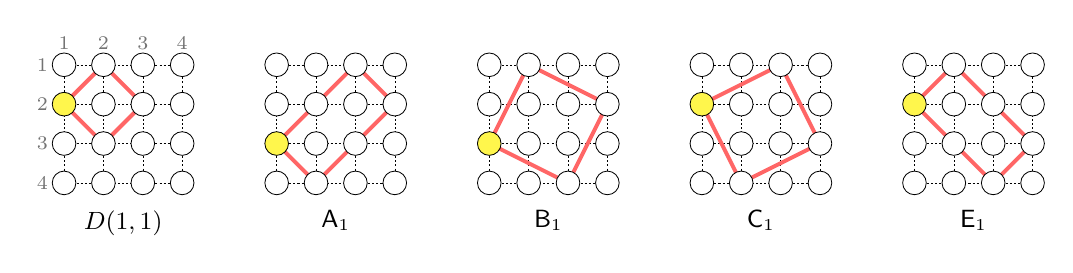
\begin{tikzpicture}[x=0.5cm,y=0.5cm,baseline=(current bounding box.north)]
  \begin{scope}[xshift=0.000cm]
    \draw[black,line width=0.20pt,dash pattern=on 0.75pt off 0.75pt] (1,-1) -- (4,-1) (1,-2) -- (4,-2) (1,-3) -- (4,-3) (1,-4) -- (4,-4) (1,-1) -- (1,-4) (2,-1) -- (2,-4) (3,-1) -- (3,-4) (4,-1) -- (4,-4);
    \draw[kred,line width=1.42pt,line join=round] (1,-2) -- (2,-1) -- (3,-2) -- (2,-3) -- cycle;
    \filldraw[fill=white,draw=black,line width=0.30pt] (1,-1) circle (0.3);
    \filldraw[fill=white,draw=black,line width=0.30pt] (2,-1) circle (0.3);
    \filldraw[fill=white,draw=black,line width=0.30pt] (3,-1) circle (0.3);
    \filldraw[fill=white,draw=black,line width=0.30pt] (4,-1) circle (0.3);
    \filldraw[fill=kyellow,draw=black,line width=0.30pt] (1,-2) circle (0.3);
    \filldraw[fill=white,draw=black,line width=0.30pt] (2,-2) circle (0.3);
    \filldraw[fill=white,draw=black,line width=0.30pt] (3,-2) circle (0.3);
    \filldraw[fill=white,draw=black,line width=0.30pt] (4,-2) circle (0.3);
    \filldraw[fill=white,draw=black,line width=0.30pt] (1,-3) circle (0.3);
    \filldraw[fill=white,draw=black,line width=0.30pt] (2,-3) circle (0.3);
    \filldraw[fill=white,draw=black,line width=0.30pt] (3,-3) circle (0.3);
    \filldraw[fill=white,draw=black,line width=0.30pt] (4,-3) circle (0.3);
    \filldraw[fill=white,draw=black,line width=0.30pt] (1,-4) circle (0.3);
    \filldraw[fill=white,draw=black,line width=0.30pt] (2,-4) circle (0.3);
    \filldraw[fill=white,draw=black,line width=0.30pt] (3,-4) circle (0.3);
    \filldraw[fill=white,draw=black,line width=0.30pt] (4,-4) circle (0.3);
    \node[lab] at (1,-0.45) {1};
    \node[lab] at (2,-0.45) {2};
    \node[lab] at (3,-0.45) {3};
    \node[lab] at (4,-0.45) {4};
    \node[lab] at (0.45,-1) {1};
    \node[lab] at (0.45,-2) {2};
    \node[lab] at (0.45,-3) {3};
    \node[lab] at (0.45,-4) {4};
    \node[capt,anchor=north] at (2.50,-4.45) {$D(1,1)$};
  \end{scope}
  \begin{scope}[xshift=2.700cm]
    \draw[black,line width=0.20pt,dash pattern=on 0.75pt off 0.75pt] (1,-1) -- (4,-1) (1,-2) -- (4,-2) (1,-3) -- (4,-3) (1,-4) -- (4,-4) (1,-1) -- (1,-4) (2,-1) -- (2,-4) (3,-1) -- (3,-4) (4,-1) -- (4,-4);
    \draw[kred,line width=1.42pt,line join=round] (1,-3) -- (2,-4) -- (4,-2) -- (3,-1) -- cycle;
    \filldraw[fill=white,draw=black,line width=0.30pt] (1,-1) circle (0.3);
    \filldraw[fill=white,draw=black,line width=0.30pt] (2,-1) circle (0.3);
    \filldraw[fill=white,draw=black,line width=0.30pt] (3,-1) circle (0.3);
    \filldraw[fill=white,draw=black,line width=0.30pt] (4,-1) circle (0.3);
    \filldraw[fill=white,draw=black,line width=0.30pt] (1,-2) circle (0.3);
    \filldraw[fill=white,draw=black,line width=0.30pt] (2,-2) circle (0.3);
    \filldraw[fill=white,draw=black,line width=0.30pt] (3,-2) circle (0.3);
    \filldraw[fill=white,draw=black,line width=0.30pt] (4,-2) circle (0.3);
    \filldraw[fill=kyellow,draw=black,line width=0.30pt] (1,-3) circle (0.3);
    \filldraw[fill=white,draw=black,line width=0.30pt] (2,-3) circle (0.3);
    \filldraw[fill=white,draw=black,line width=0.30pt] (3,-3) circle (0.3);
    \filldraw[fill=white,draw=black,line width=0.30pt] (4,-3) circle (0.3);
    \filldraw[fill=white,draw=black,line width=0.30pt] (1,-4) circle (0.3);
    \filldraw[fill=white,draw=black,line width=0.30pt] (2,-4) circle (0.3);
    \filldraw[fill=white,draw=black,line width=0.30pt] (3,-4) circle (0.3);
    \filldraw[fill=white,draw=black,line width=0.30pt] (4,-4) circle (0.3);
    \node[capt,anchor=north] at (2.50,-4.45) {$\kA_1$};
  \end{scope}
  \begin{scope}[xshift=5.400cm]
    \draw[black,line width=0.20pt,dash pattern=on 0.75pt off 0.75pt] (1,-1) -- (4,-1) (1,-2) -- (4,-2) (1,-3) -- (4,-3) (1,-4) -- (4,-4) (1,-1) -- (1,-4) (2,-1) -- (2,-4) (3,-1) -- (3,-4) (4,-1) -- (4,-4);
    \draw[kred,line width=1.42pt,line join=round] (1,-3) -- (3,-4) -- (4,-2) -- (2,-1) -- cycle;
    \filldraw[fill=white,draw=black,line width=0.30pt] (1,-1) circle (0.3);
    \filldraw[fill=white,draw=black,line width=0.30pt] (2,-1) circle (0.3);
    \filldraw[fill=white,draw=black,line width=0.30pt] (3,-1) circle (0.3);
    \filldraw[fill=white,draw=black,line width=0.30pt] (4,-1) circle (0.3);
    \filldraw[fill=white,draw=black,line width=0.30pt] (1,-2) circle (0.3);
    \filldraw[fill=white,draw=black,line width=0.30pt] (2,-2) circle (0.3);
    \filldraw[fill=white,draw=black,line width=0.30pt] (3,-2) circle (0.3);
    \filldraw[fill=white,draw=black,line width=0.30pt] (4,-2) circle (0.3);
    \filldraw[fill=kyellow,draw=black,line width=0.30pt] (1,-3) circle (0.3);
    \filldraw[fill=white,draw=black,line width=0.30pt] (2,-3) circle (0.3);
    \filldraw[fill=white,draw=black,line width=0.30pt] (3,-3) circle (0.3);
    \filldraw[fill=white,draw=black,line width=0.30pt] (4,-3) circle (0.3);
    \filldraw[fill=white,draw=black,line width=0.30pt] (1,-4) circle (0.3);
    \filldraw[fill=white,draw=black,line width=0.30pt] (2,-4) circle (0.3);
    \filldraw[fill=white,draw=black,line width=0.30pt] (3,-4) circle (0.3);
    \filldraw[fill=white,draw=black,line width=0.30pt] (4,-4) circle (0.3);
    \node[capt,anchor=north] at (2.50,-4.45) {$\kB_1$};
  \end{scope}
  \begin{scope}[xshift=8.100cm]
    \draw[black,line width=0.20pt,dash pattern=on 0.75pt off 0.75pt] (1,-1) -- (4,-1) (1,-2) -- (4,-2) (1,-3) -- (4,-3) (1,-4) -- (4,-4) (1,-1) -- (1,-4) (2,-1) -- (2,-4) (3,-1) -- (3,-4) (4,-1) -- (4,-4);
    \draw[kred,line width=1.42pt,line join=round] (1,-2) -- (2,-4) -- (4,-3) -- (3,-1) -- cycle;
    \filldraw[fill=white,draw=black,line width=0.30pt] (1,-1) circle (0.3);
    \filldraw[fill=white,draw=black,line width=0.30pt] (2,-1) circle (0.3);
    \filldraw[fill=white,draw=black,line width=0.30pt] (3,-1) circle (0.3);
    \filldraw[fill=white,draw=black,line width=0.30pt] (4,-1) circle (0.3);
    \filldraw[fill=kyellow,draw=black,line width=0.30pt] (1,-2) circle (0.3);
    \filldraw[fill=white,draw=black,line width=0.30pt] (2,-2) circle (0.3);
    \filldraw[fill=white,draw=black,line width=0.30pt] (3,-2) circle (0.3);
    \filldraw[fill=white,draw=black,line width=0.30pt] (4,-2) circle (0.3);
    \filldraw[fill=white,draw=black,line width=0.30pt] (1,-3) circle (0.3);
    \filldraw[fill=white,draw=black,line width=0.30pt] (2,-3) circle (0.3);
    \filldraw[fill=white,draw=black,line width=0.30pt] (3,-3) circle (0.3);
    \filldraw[fill=white,draw=black,line width=0.30pt] (4,-3) circle (0.3);
    \filldraw[fill=white,draw=black,line width=0.30pt] (1,-4) circle (0.3);
    \filldraw[fill=white,draw=black,line width=0.30pt] (2,-4) circle (0.3);
    \filldraw[fill=white,draw=black,line width=0.30pt] (3,-4) circle (0.3);
    \filldraw[fill=white,draw=black,line width=0.30pt] (4,-4) circle (0.3);
    \node[capt,anchor=north] at (2.50,-4.45) {$\kC_1$};
  \end{scope}
  \begin{scope}[xshift=10.800cm]
    \draw[black,line width=0.20pt,dash pattern=on 0.75pt off 0.75pt] (1,-1) -- (4,-1) (1,-2) -- (4,-2) (1,-3) -- (4,-3) (1,-4) -- (4,-4) (1,-1) -- (1,-4) (2,-1) -- (2,-4) (3,-1) -- (3,-4) (4,-1) -- (4,-4);
    \draw[kred,line width=1.42pt,line join=round] (1,-2) -- (3,-4) -- (4,-3) -- (2,-1) -- cycle;
    \filldraw[fill=white,draw=black,line width=0.30pt] (1,-1) circle (0.3);
    \filldraw[fill=white,draw=black,line width=0.30pt] (2,-1) circle (0.3);
    \filldraw[fill=white,draw=black,line width=0.30pt] (3,-1) circle (0.3);
    \filldraw[fill=white,draw=black,line width=0.30pt] (4,-1) circle (0.3);
    \filldraw[fill=kyellow,draw=black,line width=0.30pt] (1,-2) circle (0.3);
    \filldraw[fill=white,draw=black,line width=0.30pt] (2,-2) circle (0.3);
    \filldraw[fill=white,draw=black,line width=0.30pt] (3,-2) circle (0.3);
    \filldraw[fill=white,draw=black,line width=0.30pt] (4,-2) circle (0.3);
    \filldraw[fill=white,draw=black,line width=0.30pt] (1,-3) circle (0.3);
    \filldraw[fill=white,draw=black,line width=0.30pt] (2,-3) circle (0.3);
    \filldraw[fill=white,draw=black,line width=0.30pt] (3,-3) circle (0.3);
    \filldraw[fill=white,draw=black,line width=0.30pt] (4,-3) circle (0.3);
    \filldraw[fill=white,draw=black,line width=0.30pt] (1,-4) circle (0.3);
    \filldraw[fill=white,draw=black,line width=0.30pt] (2,-4) circle (0.3);
    \filldraw[fill=white,draw=black,line width=0.30pt] (3,-4) circle (0.3);
    \filldraw[fill=white,draw=black,line width=0.30pt] (4,-4) circle (0.3);
    \node[capt,anchor=north] at (2.50,-4.45) {$\kE_1$};
  \end{scope}
\end{tikzpicture}

\caption{The tilted rectangles of the $4\times m$ grid, up to translation. Each is drawn in a $4\times4$ window, and its leftmost corner $\ell$ is yellow.}
\label{fig:tilted}
\end{figure}

\begin{lemma}[tilted rectangles on narrow grids]\label{lem:tilted-narrow}
The tilted rectangles of the $3\times m$ grid are the diamonds $D(i,1)$. Those of the $4\times m$ grid are $D(i,1)$, $D(i,2)$, $\kA_i$, $\kB_i$, $\kC_i$, and $\kE_i$.
\end{lemma}

\begin{proof}
All the listed sets are rectangles. On three rows, necessarily
$b=d=1$, hence $a=c=1$ and the leftmost corner $\ell$ is in row $2$.
On four rows, $b=d=1$ again gives diamonds. The only other possibility
is $\{b,d\}=\{1,2\}=\{a,c\}$, with $\ell$ in row $1+b$.
The four choices of sides, $(2,-2),(1,1)$, $(1,-2),(2,1)$,
$(2,-1),(1,2)$, and $(1,-1),(2,2)$, give $\kA$, $\kB$, $\kC$, and $\kE$.
\end{proof}

\begin{lemma}[boundary cross]\label{lem:cross}
The first row and the first column of the $h\times m$ grid form a valid blackout, so $f(h,m)\ge h+m-1$.
\end{lemma}

\begin{proof}
Only rectangles showing at most two points need checking
(Lemma~\ref{lem:threecorners}). An axis-aligned rectangle
$\{x_1,x_2\}\times\{y_1,y_2\}$ shows $X\times Y$, where
$X=\{x_1,x_2\}\setminus\{1\}$ and $Y=\{y_1,y_2\}\setminus\{1\}$.
These recover its columns and rows, since $|X|=1$ precisely when
$1\in\{x_1,x_2\}$, and likewise for $Y$.

By Lemma~\ref{lem:leftmost}, a tilted rectangle can have only two black
corners, $\ell$ and $(x+a,r-b)$. When both are black,
$\ell=(1,1+b)$ and the shown corners are $p=(1+c,1+b+d)$ and
$q=(1+a+c,1+d)$. Their coordinates recover $a,b,c,d$. They also differ
in both coordinates, so an axis-aligned rectangle could show this pair
only if its other two corners were black, which they are not.
\end{proof}

\begin{lemma}[axis-aligned rivals]\label{lem:rival}
Let no axis-aligned rectangle be fully black. A \emph{rival} of a set $P$ of at most two white points is an axis-aligned rectangle that shows exactly $P$. The empty set has no rival, and $P$ has one exactly when it is a singleton $\{(x,r)\}$ with $\{r,s\}\in F$ for some $s\in B_x$, a vertical pair $\{(x,r),(x,s)\}$ with $\{r,s\}\in F$, a horizontal pair $\{(x,r),(z,r)\}$ with $B_x\cap B_z\ne\emptyset$, or an oblique pair $\{(x,r),(z,s)\}$ with $x\ne z$, $r\ne s$, and $(x,s),(z,r)\in S$.
\end{lemma}

\begin{proof}
A rival of $P\ne\emptyset$ has rows $\{r,s\}$ and columns $\{x,z\}$,
with every corner outside $P$ black. Reading those corners gives the
listed conditions, which force $z\ne x$ and $s\ne r$ since $(x,r)$ is white.
\end{proof}

\section{Three rows}\label{sec:three}

Take $m\ge3$ with rows $1,2,3$ downward.
The tilted rectangles are just $D(i,1)$ (Lemma~\ref{lem:tilted-narrow}).
The row bound and cross give $f(3,m)=m+2$, also obtained by the Omega
Institute~\cite{trureturing2026}. Denote the columns by $a=\{1\}$, $b=\{2\}$, $c=\{3\}$,
$A=\{1,2\}$, $B=\{1,3\}$, $C=\{2,3\}$, and $X=\{1,2,3\}$, with $a$ and $c$ \emph{outer}. A
blackout without empty columns is a \emph{word} $B_1\cdots B_m$. We also use each
double letter for its pair in $F$ (Section~\ref{sec:conv}).

\begin{proposition}[the two types]\label{prop:threeclass}
Let $S$ be a blackout of the $3\times m$ grid with $m+2$ points.
\begin{enumerate}[(a)]
\item If $S$ is valid, its word is one $X$ among singletons (type~I) or two different doubles
among singletons (type~II).
\item For every word of type~I or~II, $G_S$ is a tree, so axis-aligned rectangles have
distinct presentations.
\item There are $m3^{m-1}+\binom m2\cdot6\cdot3^{m-2}=m^23^{m-1}$ words of type~I or~II.
\end{enumerate}
\end{proposition}

\begin{proof}
(a) Lemmas~\ref{lem:H} and~\ref{lem:mantel} give $|S|=t+e(H)$,
with $t\le m$ and $e(H)\le2$. Equality forces nonempty columns and
$\sum_i(|B_i|-1)=2$, hence one triple or two doubles.
Equal doubles would give a four-cycle in $G_S$.
(b) The nonsingleton columns connect the three rows, and each
singleton adds a leaf. (c) Place the triple or ordered pair of distinct
doubles, then choose each remaining singleton.
\end{proof}

The nonsingleton letters sort \emph{candidates} into $X$, $AC$, $CA$,
$AB$, $BA$, $BC$, and $CB$, read left to right.
Use $AC_m$ for valid width-$m$ words in $AC$, and likewise for the rest.

\begin{lemma}[diamond test]\label{lem:diamond}
A candidate $S$ with pair set $F$ is valid if and only if every diamond $D(i,1)$ passes the
test below, where $P=D(i,1)\setminus S$.
\begin{enumerate}[(a)]
\item If $|P|\ge3$ or $P$ is empty, the diamond passes.
\item If $P=\{(i+1,1),(i+1,3)\}$, the diamond fails if and only if $B\in F$.
\item If $P=\{(i,2),(i+2,2)\}$, it fails if and only if $B_i\cap B_{i+2}$ meets $\{1,3\}$.
\item If $P$ is an oblique pair $\{(x,r),(z,s)\}$, it fails if and only if $(x,s),(z,r)\in S$.
\item If $P=\{(x,r)\}$, it fails if and only if $\{r,s\}\in F$ for some $s\in B_x$.
\end{enumerate}
\end{lemma}

\begin{proof}
Proposition~\ref{prop:threeclass}(b) settles axis-aligned pairs,
and Lemma~\ref{lem:threecorners} settles presentations of at least
three points. An empty diamond has no axis-aligned rival since
$G_S$ has no four-cycle. Lemma~\ref{lem:rival} gives the remaining
tests, with $B\in F$ in (b) and $\{r,s\}\in F$ in (e).
Two diamonds share at most a tip. For equal presentations, both middle
columns would need black rows $1$ and $3$, impossible in a candidate.
\end{proof}

Figure~\ref{fig:diamond} shows one passing and one failing diamond.

\begin{figure}[t]
\centering
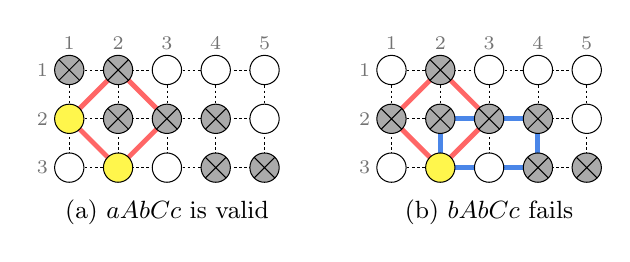
\begin{tikzpicture}[x=0.62cm,y=0.62cm,baseline=(current bounding box.north)]
  \begin{scope}[xshift=0.000cm]
    \draw[black,line width=0.25pt,dash pattern=on 0.93pt off 0.93pt] (1,-1) -- (5,-1) (1,-2) -- (5,-2) (1,-3) -- (5,-3) (1,-1) -- (1,-3) (2,-1) -- (2,-3) (3,-1) -- (3,-3) (4,-1) -- (4,-3) (5,-1) -- (5,-3);
    \draw[kred,line width=1.76pt,line join=round] (1,-2) -- (2,-1) -- (3,-2) -- (2,-3) -- cycle;
    \filldraw[fill=kgray,draw=black,line width=0.37pt] (1,-1) circle (0.3);
    \draw[black,line width=0.37pt] (0.788,-0.788) -- (1.212,-1.212) (0.788,-1.212) -- (1.212,-0.788);
    \filldraw[fill=kgray,draw=black,line width=0.37pt] (2,-1) circle (0.3);
    \draw[black,line width=0.37pt] (1.788,-0.788) -- (2.212,-1.212) (1.788,-1.212) -- (2.212,-0.788);
    \filldraw[fill=white,draw=black,line width=0.37pt] (3,-1) circle (0.3);
    \filldraw[fill=white,draw=black,line width=0.37pt] (4,-1) circle (0.3);
    \filldraw[fill=white,draw=black,line width=0.37pt] (5,-1) circle (0.3);
    \filldraw[fill=kyellow,draw=black,line width=0.37pt] (1,-2) circle (0.3);
    \filldraw[fill=kgray,draw=black,line width=0.37pt] (2,-2) circle (0.3);
    \draw[black,line width=0.37pt] (1.788,-1.788) -- (2.212,-2.212) (1.788,-2.212) -- (2.212,-1.788);
    \filldraw[fill=kgray,draw=black,line width=0.37pt] (3,-2) circle (0.3);
    \draw[black,line width=0.37pt] (2.788,-1.788) -- (3.212,-2.212) (2.788,-2.212) -- (3.212,-1.788);
    \filldraw[fill=kgray,draw=black,line width=0.37pt] (4,-2) circle (0.3);
    \draw[black,line width=0.37pt] (3.788,-1.788) -- (4.212,-2.212) (3.788,-2.212) -- (4.212,-1.788);
    \filldraw[fill=white,draw=black,line width=0.37pt] (5,-2) circle (0.3);
    \filldraw[fill=white,draw=black,line width=0.37pt] (1,-3) circle (0.3);
    \filldraw[fill=kyellow,draw=black,line width=0.37pt] (2,-3) circle (0.3);
    \filldraw[fill=white,draw=black,line width=0.37pt] (3,-3) circle (0.3);
    \filldraw[fill=kgray,draw=black,line width=0.37pt] (4,-3) circle (0.3);
    \draw[black,line width=0.37pt] (3.788,-2.788) -- (4.212,-3.212) (3.788,-3.212) -- (4.212,-2.788);
    \filldraw[fill=kgray,draw=black,line width=0.37pt] (5,-3) circle (0.3);
    \draw[black,line width=0.37pt] (4.788,-2.788) -- (5.212,-3.212) (4.788,-3.212) -- (5.212,-2.788);
    \node[lab] at (1,-0.45) {1};
    \node[lab] at (2,-0.45) {2};
    \node[lab] at (3,-0.45) {3};
    \node[lab] at (4,-0.45) {4};
    \node[lab] at (5,-0.45) {5};
    \node[lab] at (0.45,-1) {1};
    \node[lab] at (0.45,-2) {2};
    \node[lab] at (0.45,-3) {3};
    \node[capt,anchor=north] at (3.00,-3.45) {(a) $aAbCc$ is valid};
  \end{scope}
  \begin{scope}[xshift=4.092cm]
    \draw[black,line width=0.25pt,dash pattern=on 0.93pt off 0.93pt] (1,-1) -- (5,-1) (1,-2) -- (5,-2) (1,-3) -- (5,-3) (1,-1) -- (1,-3) (2,-1) -- (2,-3) (3,-1) -- (3,-3) (4,-1) -- (4,-3) (5,-1) -- (5,-3);
    \draw[kblue,line width=1.76pt,line join=round] (2,-2) -- (4,-2) -- (4,-3) -- (2,-3) -- cycle;
    \draw[kred,line width=1.76pt,line join=round] (1,-2) -- (2,-1) -- (3,-2) -- (2,-3) -- cycle;
    \filldraw[fill=white,draw=black,line width=0.37pt] (1,-1) circle (0.3);
    \filldraw[fill=kgray,draw=black,line width=0.37pt] (2,-1) circle (0.3);
    \draw[black,line width=0.37pt] (1.788,-0.788) -- (2.212,-1.212) (1.788,-1.212) -- (2.212,-0.788);
    \filldraw[fill=white,draw=black,line width=0.37pt] (3,-1) circle (0.3);
    \filldraw[fill=white,draw=black,line width=0.37pt] (4,-1) circle (0.3);
    \filldraw[fill=white,draw=black,line width=0.37pt] (5,-1) circle (0.3);
    \filldraw[fill=kgray,draw=black,line width=0.37pt] (1,-2) circle (0.3);
    \draw[black,line width=0.37pt] (0.788,-1.788) -- (1.212,-2.212) (0.788,-2.212) -- (1.212,-1.788);
    \filldraw[fill=kgray,draw=black,line width=0.37pt] (2,-2) circle (0.3);
    \draw[black,line width=0.37pt] (1.788,-1.788) -- (2.212,-2.212) (1.788,-2.212) -- (2.212,-1.788);
    \filldraw[fill=kgray,draw=black,line width=0.37pt] (3,-2) circle (0.3);
    \draw[black,line width=0.37pt] (2.788,-1.788) -- (3.212,-2.212) (2.788,-2.212) -- (3.212,-1.788);
    \filldraw[fill=kgray,draw=black,line width=0.37pt] (4,-2) circle (0.3);
    \draw[black,line width=0.37pt] (3.788,-1.788) -- (4.212,-2.212) (3.788,-2.212) -- (4.212,-1.788);
    \filldraw[fill=white,draw=black,line width=0.37pt] (5,-2) circle (0.3);
    \filldraw[fill=white,draw=black,line width=0.37pt] (1,-3) circle (0.3);
    \filldraw[fill=kyellow,draw=black,line width=0.37pt] (2,-3) circle (0.3);
    \filldraw[fill=white,draw=black,line width=0.37pt] (3,-3) circle (0.3);
    \filldraw[fill=kgray,draw=black,line width=0.37pt] (4,-3) circle (0.3);
    \draw[black,line width=0.37pt] (3.788,-2.788) -- (4.212,-3.212) (3.788,-3.212) -- (4.212,-2.788);
    \filldraw[fill=kgray,draw=black,line width=0.37pt] (5,-3) circle (0.3);
    \draw[black,line width=0.37pt] (4.788,-2.788) -- (5.212,-3.212) (4.788,-3.212) -- (5.212,-2.788);
    \node[lab] at (1,-0.45) {1};
    \node[lab] at (2,-0.45) {2};
    \node[lab] at (3,-0.45) {3};
    \node[lab] at (4,-0.45) {4};
    \node[lab] at (5,-0.45) {5};
    \node[lab] at (0.45,-1) {1};
    \node[lab] at (0.45,-2) {2};
    \node[lab] at (0.45,-3) {3};
    \node[capt,anchor=north] at (3.00,-3.45) {(b) $bAbCc$ fails};
  \end{scope}
\end{tikzpicture}

\caption{The diamond test. (a) In $aAbCc$ the diamond $D(1,1)$ shows the oblique pair $(1,2),(2,3)$, which has no rival since $(1,3)$ is white. (b) In $bAbCc$ it shows only $(2,3)$, and so does the axis-aligned rectangle on columns $2,4$ and rows $2,3$, since $2\in B_2$ and $C\in F$ (Lemma~\ref{lem:diamond}(e)).}
\label{fig:diamond}
\end{figure}

A \emph{window} is three consecutive letters, in columns $i$ to $i+2$.
It \emph{passes} or \emph{fails} with $D(i,1)$.
Its \emph{tips} $(i,2)$ and $(i+2,2)$ are black exactly when their letters
are $b$, $A$, $C$, or $X$.

\begin{lemma}[singleton dichotomy]\label{lem:dichotomy}
In a candidate, a window of three singletons fails if and only if $B\in F$ and it is
$bab$, $bbb$, or $bcb$.
\end{lemma}

\begin{proof}
With two black tips, the vertical pair or one middle-column corner
remains. Tests (b) and (e) reject exactly when $B\in F$.
With one black tip, three corners remain or test (d) passes because
$(i+1,2)$ is white. With neither, at least three corners remain.
\end{proof}

\begin{lemma}[six of nine in the class $\{A,C\}$]\label{lem:sixofnine}
Let $S$ be a candidate with $F=\{A,C\}$, and let $s,t$ be singletons.
\begin{enumerate}[(a)]
\item A window $sAt$ fails if and only if $st$ is $bb$, $bc$, or $cb$, also for $t=C$ read
as $t=b$.
\item A window $sCt$ fails if and only if $st$ is $bb$, $ba$, or $ab$.
\item A window with one double, at a tip, passes.
\end{enumerate}
\end{lemma}

\begin{proof}
(a) Only $(i+1,3)$ is white in the middle column.
The right tip $(i+2,2)$ is black for $t\in\{b,C\}$.
With both tips black, test (e) fails since $2\in B_{i+1}$ and $C\in F$.
With just the right tip black, the pair $(i,2),(i+1,3)$ fails test (d)
exactly for $s=c$. The other tip is symmetric. With neither black,
three corners show. (b) Reflect across the middle row.
(c) Apply Lemma~\ref{lem:dichotomy} to $Ast$ with the left tip
already black. No case fails since $B\notin F$.
Reflection and reversal give the remaining positions.
\end{proof}

A word in $AC_m$ has form $UAVCW$, with singleton strings $U$, $V$,
and $W$. By the diamond test it is enough that every window passes.
Set $G_{AC}(z)=\sum_{m\ge2}|AC_m|z^m$. Define $G_{AB}$ by counting
$UAVBW$, and $G_X(z)=\sum_{m\ge1}|X_m|z^m$ by counting $UXW$.
Write $\Phi=1-3z$. A nonempty singleton string with a specified letter
next to a double contributes $z/\Phi$.

\begin{proposition}[the class $\{A,C\}$]\label{prop:threeGAC}
The generating function of $AC$ is
\begin{equation}\label{eq:GAC}
G_{AC}(z)=\frac{z^2-4z^3+10z^4-8z^5-3z^6}{(1-3z)^3},
\end{equation}
and
\begin{equation}\label{eq:GACcoef}
|AC_m|=2(m-1)(3m+2)3^{m-5}\qquad(m\ge4).
\end{equation}
\end{proposition}

\begin{proof}
Lemma~\ref{lem:sixofnine}(a) and the half turn allow $tAC$ only for
$t=a$ and $ACt$ only for $t=c$. Each $AtC$ passes tests (b) and (e).
Lemmas~\ref{lem:dichotomy} and~\ref{lem:sixofnine}(c) leave only
windows centered on a double.

Split according to the gap $V$. With no gap, a nonempty $U$ must end in
$a$ and a nonempty $W$ must start in $c$, contributing $z^2(1+z/\Phi)^2$.
For $V=t$, the allowed last letters of $U$ number $p_t=3,1,2$, and the
allowed first letters of $W$ number $q_t=2,1,3$, for $t=a,b,c$.
Thus $\sum p_t=\sum q_t=6$ and $\sum p_tq_t=13$, giving
$z^3\sum_t(1+p_tz/\Phi)(1+q_tz/\Phi)=z^3(3+12z/\Phi+13z^2/\Phi^2)$.
For $|V|\ge2$, each end contributes $3+6z/\Phi$ (a lone endpoint letter,
or one of six passing pairs). The unrestricted middle contributes
$1/\Phi$, so this case gives $9z^4(1-z)^2/\Phi^3$.
Adding proves~\eqref{eq:GAC}. Extract coefficients using
$[z^m]z^k\Phi^{-3}=\binom{m-k+2}23^{m-k}$ to obtain~\eqref{eq:GACcoef}.
\end{proof}

\begin{theorem}[the number of three-row optima]\label{thm:threecount}
Let $E_m$ count the optima of the $3\times m$ grid with a column black in rows $1$ and $3$
(\seqnum{A398448}). For $m\ge4$,
\begin{equation}\label{eq:threecount}
a_3(m)=4(m-1)(3m+2)3^{m-5}+E_m.
\end{equation}
\end{theorem}

\begin{proof}
A column black in rows $1$ and $3$ must be $B$ or $X$.
Proposition~\ref{prop:threeclass}(a) therefore identifies these optima
with the classes other than $AC$ and $CA$. Reversing columns pairs
$AC$, $AB$, and $BC$ with $CA$, $BA$, and $CB$, respectively.
Reflection across the middle row also pairs $AB$ with $CB$. Hence
\begin{equation}\label{eq:classsum}
a_3(m)=2|AC_m|+4|AB_m|+|X_m|=2|AC_m|+E_m\qquad(m\ge3),
\end{equation}
and substituting~\eqref{eq:GACcoef} gives~\eqref{eq:threecount}.
\end{proof}

\subsection{The generating function}

Put $L=1-2z-2z^2$, $N=1+2z^2$, and $\Psi=LN$.

\begin{theorem}[three-row generating function, parts (b) and (c) computer-assisted]\label{thm:threegf}
\leavevmode
\begin{enumerate}[(a)]
\item The series $\sum_{m\ge3}a_3(m)z^m$ equals $2G_{AC}+4G_{AB}+G_X-z-12z^2$, with
$G_{AB}$ and $G_X$ from Propositions~\ref{prop:GAB} and~\ref{prop:GX}, of denominators
dividing $\Psi^3$ and $\Psi^2$.
\item Its reduced denominator is exactly $Q=\Phi^3L^3N^3$.
\item With
\begin{align*}
P(z)={}&z-3z^2-34z^3+228z^4-641z^5+1307z^6-2186z^7\\
&+2056z^8-236z^9-1060z^{10}+2584z^{11}-4264z^{12}\\
&-1440z^{13}+704z^{14}-1024z^{15}+2080z^{16}+2176z^{17}+384z^{18},
\end{align*}
we have
\begin{equation}\label{eq:PQ}
\sum_{m\ge3}a_3(m)z^m=\frac{P(z)}{Q(z)}-z-12z^2.
\end{equation}
\end{enumerate}
\end{theorem}

\begin{proof}
For (a), sum~\eqref{eq:classsum}, removing widths one and two by
subtracting $z+12z^2$. Part (b) is proved in Section~\ref{app:threegf}.
For (c), exact algebra in SymPy~\cite{sympy2017} gives $P$.
The script \nolinkurl{three_row_closed_form_check.py} independently
checks~\eqref{eq:PQ} against a transfer matrix through width $100$.
\end{proof}

Let $\rho=1+\sqrt3$ and $\sigma=1-\sqrt3$.

\begin{theorem}[three-row closed form, computer-assisted exact algebra]\label{thm:threeclosed}
For every $m\ge3$,
\begin{equation}\label{eq:Eclosed}
E_m=p_+(m)\rho^m+p_-(m)\sigma^m+\eta_m,
\end{equation}
where $432\,p_\pm(m)=(19\pm11\sqrt3)m^2+(61\pm41\sqrt3)m+104\pm28\sqrt3$ and $\eta_m=(-2)^{\lfloor m/2\rfloor}\,\kappa(m)$ with $\kappa(m)=(2m^2+41m-104)/216$ for even $m$ and
$\kappa(m)=(7m^2-32m-175)/432$ for odd $m$. Hence $E_m\sim\frac{19+11\sqrt3}{432}m^2\rho^m$. The hand proof gives $E_m>0$ and
\begin{equation}\label{eq:asymp1}
a_3(m)=\frac4{81}m^23^m-\frac4{243}(m+2)3^m+O(m^2\rho^m).
\end{equation}
\end{theorem}

\begin{proof}
Equation~\eqref{eq:classsum} makes $E_m$ the coefficient of $z^m$
in $4G_{AB}+G_X$, with denominator dividing $L^3N^3$.
The possible poles are $1/\rho$, $1/\sigma$, and $\pm1/(i\sqrt2)$,
each of order at most three. Apart from a polynomial part of degree one,
their coefficients have the form~\eqref{eq:Eclosed}.
Exact algebra determines the twelve rational constants. Both sides obey the order-$12$ recurrence
from $L^3N^3$ for $m=14$ onward and agree at $m=2,\dots,13$.
The leading term follows from $|\sigma|<1$ and
$|\eta_m|=O(m^22^{m/2})$. For the hand bound, the pole $1/\rho$
of least modulus gives $E_m=O(m^2\rho^m)$, which yields~\eqref{eq:asymp1}
through~\eqref{eq:threecount}. Finally, the boundary cross has word
$Xa\cdots a$ (Lemma~\ref{lem:cross}), so $E_m>0$.
\end{proof}

\subsection{\texorpdfstring{The classes $AB$ and $X$}{The classes AB and X}}\label{app:threegf}

It remains to count $X$ and $AB$ and rule out cancellation in
Theorem~\ref{thm:threegf}(b). Keep $\Psi=LN=1-2z-4z^3-4z^4$.
A \emph{restricted} singleton string has no two $b$ letters at distance
two. Reversal and reflection carry $AB$ to $BA$, $BC$, and $CB$.

\begin{lemma}[forbidden windows in the classes containing $B$]\label{lem:threewindows}
In classes $AB$ and $X$, the table lists exactly the failing windows.
Here $s$ is any singleton.
\begin{center}\small
\begin{tabular}{@{}lll@{}}
\toprule
class & windows & forbidden \\
\midrule
$AB$, $X$ & singletons only & $bsb$ \\
$AB$ & one double & $bsA$, $Asb$, $bAb$, $bAc$, $cAb$, $aBa$, $aBb$, $bBa$, $cBc$ \\
 & two doubles & $bAB$, $ABa$ \\
$X$ & one triple & $bsX$, $Xsb$, $aXa$, $aXb$, $bXa$, $bXc$, $cXb$, $cXc$ \\
\bottomrule
\end{tabular}
\end{center}
\end{lemma}

\begin{proof}
Lemma~\ref{lem:dichotomy} handles singleton windows.
For $sAt$, use Lemma~\ref{lem:sixofnine}(a), also rejecting $bAb$
by test (e) since $B\in F$.
In $sBt$ or $sXt$, the middle corners are black. For $s=t=b$ the
diamond is empty. For outer letters, test (c) fails exactly for $s=t$.
For $s=b\ne t$, only $(i+2,2)$ shows, and test (e) fails exactly
when $\{2,t\}\in F$.
In $uAB$, the black corners $(i+2,3),(i+1,2)$ make test (d) fail
for $u=b$, while otherwise three corners show.
In $ABw$, $w=b$ gives an empty diamond, and test (e) rejects $w=a$.
Tests (b) and (e) exclude $Asb$ and $Xsb$.
Other left-tip windows show three corners or need the white point
$(i+1,2)$ for an oblique rival. Reflect for the other cases.
\end{proof}

Encode outer letters by bit $0$ with weight $2$, and $b$ by bit $1$.
Let $h_{ij}$ count continuations after $i,j$, forbidding $b$ after $1,j$.
Read each run $w_1\cdots w_n$, $n\ge1$, away from its double.
Let $g_0,g_1$ count a prescribed outer first letter and $w_1=b$,
and $u,v$ the same with $w_2$ outer if present.
A fictitious preceding letter, outer for $g$ and $b$ for $u,v$,
gives $(g_0,g_1,u,v)=z(h_{00},h_{01},h_{10},h_{11})$.
The recurrence solves to
\begin{equation}\label{eq:runs}
\Psi g_0=z(1+z+3z^2+2z^3),\ \ \Psi g_1=z(1+z),\ \ \Psi u=z(1+2z^2+2z^3),\ \ \Psi v=z.
\end{equation}

\begin{proposition}[the triple class]\label{prop:GX}
With $u$ and $v$ as in~\eqref{eq:runs}, $G_X(z)=z\bigl(1+4u+2v+2u^2+v^2\bigr)$, and its
denominator divides $\Psi^2$.
\end{proposition}

\begin{proof}
In $UXW$, both runs are restricted. Forbidding $bsX$ and $Xsb$
makes the second letter from $X$ outer. A single nonempty side gives
$2u+v$, on either side. Two nonempty sides allow neighbor pairs
$(a,c)$, $(b,b)$, and $(c,a)$, contributing $2u^2+v^2$.
\end{proof}

In $UAVBW$, all singleton runs are restricted. Reading outward,
$U$ from $A$ uses $u$ or $v$, and $W$ from $B$ uses $g_0$ or $g_1$
(Lemma~\ref{lem:threewindows}). Include empty runs in $\ell_t$ and $r_t$
when $t$ follows $A$ or precedes $B$. The double-centered windows give
\begin{equation}\label{eq:lr}
(\ell_a,\ell_b,\ell_c)=(1+2u+v,1+u,1+2u),\ (r_a,r_b,r_c)=(1+g_0,1+g_0+g_1,1+g_0+g_1).
\end{equation}
We also need the final bit. For $s\in\{00,10\}$, let $J_{s\beta}$
count continuations from $s$ ending in $\beta$, assigning the empty
continuation to $\beta=0$. The same recurrence gives the matrix below,
with rows indexed by $s$ and columns by $\beta$
\begin{equation}\label{eq:J}
J=\frac1\Psi\begin{pmatrix}1+2z^2+2z^3&z+z^2\\1&2z^2+2z^3\end{pmatrix}.
\end{equation}

\begin{proposition}[the class $\{A,B\}$, polynomial form computer-assisted]\label{prop:GAB}
With~\eqref{eq:runs} to~\eqref{eq:J},
\begin{equation}\label{eq:GAB}
\begin{aligned}
G_{AB}(z)={}&z^2(1+2u)(1+g_0+g_1)+z^3(\ell_ar_a+\ell_br_b+\ell_cr_c)\\
&+z^4\,(\ell_a+\ell_c,\ \ell_b)\,J\,(r_a+r_c,\ 2r_b)^{T}.
\end{aligned}
\end{equation}
Moreover $G_{AB}=P_B/\Psi^3$ with
\begin{equation}\label{eq:PB}
P_B(z)=z^2(1+z)(1+z^2-3z^3+4z^6+4z^7).
\end{equation}
\end{proposition}

\begin{proof}
Let $k$ be the length of $V$. For $k=0$, the boundary windows
$uAB$ and $ABw$ require $u\ne b$ and $w\ne a$, giving the first term.
For $k=1$, $AtB$ always passes, while $uAt$ and $tBw$ contribute
$\ell_tr_t$.

For $k\ge2$, $Av_1v_2$ forces $v_2$ to be outer, and
$v_{k-1}v_kB$ always passes. The remaining string $v_3\cdots v_k$
continues from bits $00$ or $10$, according as $v_1$ is outer or $b$,
with boundary weight $\ell_{v_1}r_{v_k}$. The vector entry $r_a+r_c$
already counts the two outer choices for $v_k$. Thus for $k\ge3$,
the outer-letter weight $2$ in $J$, and the factor $2$ in $2r_b$,
account for the two choices of $v_2$. The constant term of $J$ handles
$k=2$. This gives~\eqref{eq:GAB}, and exact algebra gives~\eqref{eq:PB}.
\end{proof}

\begin{proof}[Proof of Theorem~\ref{thm:threegf}(b)]
The denominator divides $\Phi^3\Psi^3=Q$ by part (a).
Its factors share no roots, since $\Psi(\frac13)\ne0$ and
$L-N=-2z-4z^2$ vanishes only where $N\ne0$.
At $z=\frac13$, $G_{AC}$ alone has a triple pole, its numerator
being $\frac4{81}$. At roots of $\Psi$, the remainders
$P_B\bmod L=\frac z2$ and $P_B\bmod N=\frac14-\frac z2$
are nonzero. Thus $G_{AB}$ has triple poles there, which neither
the double poles of $G_X$ nor the regular $G_{AC}$ can cancel.
\end{proof}

\begin{remark}[optima up to symmetry]\label{rem:threeorbits}
Counting up to row reflection and column reversal gives $o_3(m)$,
with first values $15$, $58$, $227$, $864$, $3190$, and $11502$
for widths $3$ to $8$ (\seqnum{A401226}). Burnside's lemma says that
$4o_3(m)$ equals $a_3(m)$ plus the fixed counts of the three nonidentity
symmetries. Row reflection allows only $b$, $B$, and $X$.
An optimum must therefore have one $X$ and otherwise $b$.
For $m\ge4$, one of $Xbb$, $bbX$, or $bbb$ occurs and fails
(Lemmas~\ref{lem:diamond}(b) and~\ref{lem:dichotomy}).
The only fixed optimum is $bXb$.

For the half turn, put $m=2k$ or $m=2k+1$.
It reverses the word and exchanges $A$ with $C$ and $a$ with $c$.
A fixed two-double word has $A$ and $C$ in mirror columns $j\le k$
and $m+1-j$, with $b$ at the center for odd $m$.
The first $k$ letters determine the rest. Only the windows centered
on $A$ and $C$ can fail (the proof of Proposition~\ref{prop:threeGAC}),
and these are mirror images. Lemma~\ref{lem:sixofnine}(a) leaves
$3^{k-1}$ words in $AC$ when $j=1$, $3^{k-2}$ when $j=k\ge2$,
and $2\cdot3^{k-2}$ when $1<j<k$. The count in $CA$ is equal.
Summing gives $4k3^{k-2}$ for $k\ge2$.
At $m=3$ there are just $AbC$ and $CbA$. Their combined series is
$W=2z^3+\frac49(1+z)\bigl(3z^2(1-3z^2)^{-2}-3z^2\bigr)$.

Column reversal forces a palindrome. Every noncentral letter is
repeated, so a fixed optimum must have odd width and form
$UXU^{\mathrm{rev}}$. The middle window $tXt$ requires $t=b$,
and the forbidden windows $bsX$ and $Xsb$ force the next letter
outward to be outer (Lemma~\ref{lem:threewindows}). Thus $U$ is
counted by $v$ in~\eqref{eq:runs}.
For a half-turn-fixed triple word $UX\iota(U^{\mathrm{rev}})$,
where $\iota$ reflects rows, the allowed middle pairs are
$(a,c)$, $(b,b)$, and $(c,a)$, giving $2u+v$ for $U$.
Combine the contribution $z^3$ of $bXb$, the paired-run contribution
$2z\bigl(u(z^2)+v(z^2)\bigr)$, and the two-double contribution $W$ to get
\begin{align*}
4\sum_{m\ge3}o_3(m)z^m={}&\sum_{m\ge3}a_3(m)z^m+z^3+\frac{4z^3(1+z^4+z^6)}{M(1+2z^4)}\\
&+\frac{2z^3(1-z)(1+5z+3z^2-3z^3)}{(1-3z^2)^2},
\end{align*}
Here $M=1-2z^2-2z^4$, so $\Psi(z^2)=M(1+2z^4)$.
The independent check \nolinkurl{three_row_orbits.py} agrees with the
fixed counts through width $24$ and the orbit counts $o_3(m)$ for $m\le10$.
\end{remark}

\section{Four rows}\label{sec:four}

\begin{theorem}[four rows]\label{thm:fourvalue}
For every $m\ge6$ we have $f(4,m)=m+4$.
\end{theorem}

To attain the upper bound of Theorem~\ref{thm:rowbound}, use
\begin{equation}\label{eq:fourS}
S=\{(i,1):2\le i\le m-1\}\cup\{(m-1,2),(m,2),(1,3),(2,3),(1,4),(m,4)\}.
\end{equation}
Here $|S|=m+4$ and $G_S$ is the eight-cycle $r_1\,c_2\,r_3\,c_1\,r_4\,c_m\,r_2\,c_{m-1}$ with leaves $c_3,\ldots,c_{m-2}$ on $r_1$ (Figure~\ref{fig:four}).

\begin{figure}[t]
\centering
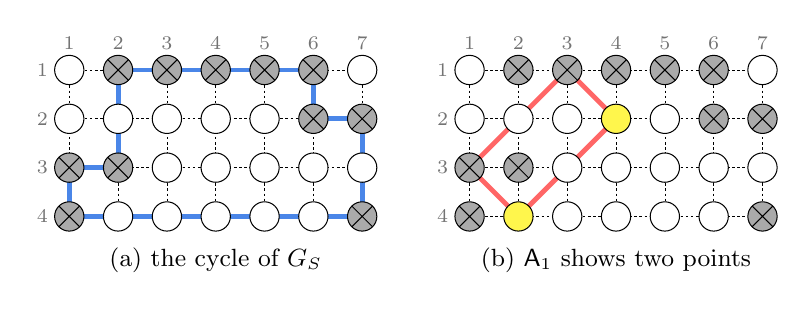
\begin{tikzpicture}[x=0.62cm,y=0.62cm,baseline=(current bounding box.north)]
  \begin{scope}[xshift=0.000cm]
    \draw[black,line width=0.25pt,dash pattern=on 0.93pt off 0.93pt] (1,-1) -- (7,-1) (1,-2) -- (7,-2) (1,-3) -- (7,-3) (1,-4) -- (7,-4) (1,-1) -- (1,-4) (2,-1) -- (2,-4) (3,-1) -- (3,-4) (4,-1) -- (4,-4) (5,-1) -- (5,-4) (6,-1) -- (6,-4) (7,-1) -- (7,-4);
    \draw[kblue,line width=1.76pt,line join=round] (2,-1) -- (6,-1) -- (6,-2) -- (7,-2) -- (7,-4) -- (1,-4) -- (1,-3) -- (2,-3) -- cycle;
    \filldraw[fill=white,draw=black,line width=0.37pt] (1,-1) circle (0.3);
    \filldraw[fill=kgray,draw=black,line width=0.37pt] (2,-1) circle (0.3);
    \draw[black,line width=0.37pt] (1.788,-0.788) -- (2.212,-1.212) (1.788,-1.212) -- (2.212,-0.788);
    \filldraw[fill=kgray,draw=black,line width=0.37pt] (3,-1) circle (0.3);
    \draw[black,line width=0.37pt] (2.788,-0.788) -- (3.212,-1.212) (2.788,-1.212) -- (3.212,-0.788);
    \filldraw[fill=kgray,draw=black,line width=0.37pt] (4,-1) circle (0.3);
    \draw[black,line width=0.37pt] (3.788,-0.788) -- (4.212,-1.212) (3.788,-1.212) -- (4.212,-0.788);
    \filldraw[fill=kgray,draw=black,line width=0.37pt] (5,-1) circle (0.3);
    \draw[black,line width=0.37pt] (4.788,-0.788) -- (5.212,-1.212) (4.788,-1.212) -- (5.212,-0.788);
    \filldraw[fill=kgray,draw=black,line width=0.37pt] (6,-1) circle (0.3);
    \draw[black,line width=0.37pt] (5.788,-0.788) -- (6.212,-1.212) (5.788,-1.212) -- (6.212,-0.788);
    \filldraw[fill=white,draw=black,line width=0.37pt] (7,-1) circle (0.3);
    \filldraw[fill=white,draw=black,line width=0.37pt] (1,-2) circle (0.3);
    \filldraw[fill=white,draw=black,line width=0.37pt] (2,-2) circle (0.3);
    \filldraw[fill=white,draw=black,line width=0.37pt] (3,-2) circle (0.3);
    \filldraw[fill=white,draw=black,line width=0.37pt] (4,-2) circle (0.3);
    \filldraw[fill=white,draw=black,line width=0.37pt] (5,-2) circle (0.3);
    \filldraw[fill=kgray,draw=black,line width=0.37pt] (6,-2) circle (0.3);
    \draw[black,line width=0.37pt] (5.788,-1.788) -- (6.212,-2.212) (5.788,-2.212) -- (6.212,-1.788);
    \filldraw[fill=kgray,draw=black,line width=0.37pt] (7,-2) circle (0.3);
    \draw[black,line width=0.37pt] (6.788,-1.788) -- (7.212,-2.212) (6.788,-2.212) -- (7.212,-1.788);
    \filldraw[fill=kgray,draw=black,line width=0.37pt] (1,-3) circle (0.3);
    \draw[black,line width=0.37pt] (0.788,-2.788) -- (1.212,-3.212) (0.788,-3.212) -- (1.212,-2.788);
    \filldraw[fill=kgray,draw=black,line width=0.37pt] (2,-3) circle (0.3);
    \draw[black,line width=0.37pt] (1.788,-2.788) -- (2.212,-3.212) (1.788,-3.212) -- (2.212,-2.788);
    \filldraw[fill=white,draw=black,line width=0.37pt] (3,-3) circle (0.3);
    \filldraw[fill=white,draw=black,line width=0.37pt] (4,-3) circle (0.3);
    \filldraw[fill=white,draw=black,line width=0.37pt] (5,-3) circle (0.3);
    \filldraw[fill=white,draw=black,line width=0.37pt] (6,-3) circle (0.3);
    \filldraw[fill=white,draw=black,line width=0.37pt] (7,-3) circle (0.3);
    \filldraw[fill=kgray,draw=black,line width=0.37pt] (1,-4) circle (0.3);
    \draw[black,line width=0.37pt] (0.788,-3.788) -- (1.212,-4.212) (0.788,-4.212) -- (1.212,-3.788);
    \filldraw[fill=white,draw=black,line width=0.37pt] (2,-4) circle (0.3);
    \filldraw[fill=white,draw=black,line width=0.37pt] (3,-4) circle (0.3);
    \filldraw[fill=white,draw=black,line width=0.37pt] (4,-4) circle (0.3);
    \filldraw[fill=white,draw=black,line width=0.37pt] (5,-4) circle (0.3);
    \filldraw[fill=white,draw=black,line width=0.37pt] (6,-4) circle (0.3);
    \filldraw[fill=kgray,draw=black,line width=0.37pt] (7,-4) circle (0.3);
    \draw[black,line width=0.37pt] (6.788,-3.788) -- (7.212,-4.212) (6.788,-4.212) -- (7.212,-3.788);
    \node[lab] at (1,-0.45) {1};
    \node[lab] at (2,-0.45) {2};
    \node[lab] at (3,-0.45) {3};
    \node[lab] at (4,-0.45) {4};
    \node[lab] at (5,-0.45) {5};
    \node[lab] at (6,-0.45) {6};
    \node[lab] at (7,-0.45) {7};
    \node[lab] at (0.45,-1) {1};
    \node[lab] at (0.45,-2) {2};
    \node[lab] at (0.45,-3) {3};
    \node[lab] at (0.45,-4) {4};
    \node[capt,anchor=north] at (4.00,-4.45) {(a) the cycle of $G_S$};
  \end{scope}
  \begin{scope}[xshift=5.084cm]
    \draw[black,line width=0.25pt,dash pattern=on 0.93pt off 0.93pt] (1,-1) -- (7,-1) (1,-2) -- (7,-2) (1,-3) -- (7,-3) (1,-4) -- (7,-4) (1,-1) -- (1,-4) (2,-1) -- (2,-4) (3,-1) -- (3,-4) (4,-1) -- (4,-4) (5,-1) -- (5,-4) (6,-1) -- (6,-4) (7,-1) -- (7,-4);
    \draw[kred,line width=1.76pt,line join=round] (1,-3) -- (2,-4) -- (4,-2) -- (3,-1) -- cycle;
    \filldraw[fill=white,draw=black,line width=0.37pt] (1,-1) circle (0.3);
    \filldraw[fill=kgray,draw=black,line width=0.37pt] (2,-1) circle (0.3);
    \draw[black,line width=0.37pt] (1.788,-0.788) -- (2.212,-1.212) (1.788,-1.212) -- (2.212,-0.788);
    \filldraw[fill=kgray,draw=black,line width=0.37pt] (3,-1) circle (0.3);
    \draw[black,line width=0.37pt] (2.788,-0.788) -- (3.212,-1.212) (2.788,-1.212) -- (3.212,-0.788);
    \filldraw[fill=kgray,draw=black,line width=0.37pt] (4,-1) circle (0.3);
    \draw[black,line width=0.37pt] (3.788,-0.788) -- (4.212,-1.212) (3.788,-1.212) -- (4.212,-0.788);
    \filldraw[fill=kgray,draw=black,line width=0.37pt] (5,-1) circle (0.3);
    \draw[black,line width=0.37pt] (4.788,-0.788) -- (5.212,-1.212) (4.788,-1.212) -- (5.212,-0.788);
    \filldraw[fill=kgray,draw=black,line width=0.37pt] (6,-1) circle (0.3);
    \draw[black,line width=0.37pt] (5.788,-0.788) -- (6.212,-1.212) (5.788,-1.212) -- (6.212,-0.788);
    \filldraw[fill=white,draw=black,line width=0.37pt] (7,-1) circle (0.3);
    \filldraw[fill=white,draw=black,line width=0.37pt] (1,-2) circle (0.3);
    \filldraw[fill=white,draw=black,line width=0.37pt] (2,-2) circle (0.3);
    \filldraw[fill=white,draw=black,line width=0.37pt] (3,-2) circle (0.3);
    \filldraw[fill=kyellow,draw=black,line width=0.37pt] (4,-2) circle (0.3);
    \filldraw[fill=white,draw=black,line width=0.37pt] (5,-2) circle (0.3);
    \filldraw[fill=kgray,draw=black,line width=0.37pt] (6,-2) circle (0.3);
    \draw[black,line width=0.37pt] (5.788,-1.788) -- (6.212,-2.212) (5.788,-2.212) -- (6.212,-1.788);
    \filldraw[fill=kgray,draw=black,line width=0.37pt] (7,-2) circle (0.3);
    \draw[black,line width=0.37pt] (6.788,-1.788) -- (7.212,-2.212) (6.788,-2.212) -- (7.212,-1.788);
    \filldraw[fill=kgray,draw=black,line width=0.37pt] (1,-3) circle (0.3);
    \draw[black,line width=0.37pt] (0.788,-2.788) -- (1.212,-3.212) (0.788,-3.212) -- (1.212,-2.788);
    \filldraw[fill=kgray,draw=black,line width=0.37pt] (2,-3) circle (0.3);
    \draw[black,line width=0.37pt] (1.788,-2.788) -- (2.212,-3.212) (1.788,-3.212) -- (2.212,-2.788);
    \filldraw[fill=white,draw=black,line width=0.37pt] (3,-3) circle (0.3);
    \filldraw[fill=white,draw=black,line width=0.37pt] (4,-3) circle (0.3);
    \filldraw[fill=white,draw=black,line width=0.37pt] (5,-3) circle (0.3);
    \filldraw[fill=white,draw=black,line width=0.37pt] (6,-3) circle (0.3);
    \filldraw[fill=white,draw=black,line width=0.37pt] (7,-3) circle (0.3);
    \filldraw[fill=kgray,draw=black,line width=0.37pt] (1,-4) circle (0.3);
    \draw[black,line width=0.37pt] (0.788,-3.788) -- (1.212,-4.212) (0.788,-4.212) -- (1.212,-3.788);
    \filldraw[fill=kyellow,draw=black,line width=0.37pt] (2,-4) circle (0.3);
    \filldraw[fill=white,draw=black,line width=0.37pt] (3,-4) circle (0.3);
    \filldraw[fill=white,draw=black,line width=0.37pt] (4,-4) circle (0.3);
    \filldraw[fill=white,draw=black,line width=0.37pt] (5,-4) circle (0.3);
    \filldraw[fill=white,draw=black,line width=0.37pt] (6,-4) circle (0.3);
    \filldraw[fill=kgray,draw=black,line width=0.37pt] (7,-4) circle (0.3);
    \draw[black,line width=0.37pt] (6.788,-3.788) -- (7.212,-4.212) (6.788,-4.212) -- (7.212,-3.788);
    \node[lab] at (1,-0.45) {1};
    \node[lab] at (2,-0.45) {2};
    \node[lab] at (3,-0.45) {3};
    \node[lab] at (4,-0.45) {4};
    \node[lab] at (5,-0.45) {5};
    \node[lab] at (6,-0.45) {6};
    \node[lab] at (7,-0.45) {7};
    \node[lab] at (0.45,-1) {1};
    \node[lab] at (0.45,-2) {2};
    \node[lab] at (0.45,-3) {3};
    \node[lab] at (0.45,-4) {4};
    \node[capt,anchor=north] at (4.00,-4.45) {(b) $\kA_1$ shows two points};
  \end{scope}
\end{tikzpicture}

\caption{The blackout~\eqref{eq:fourS} for $m=7$. (a) Its row-column graph is an eight-cycle, traced through the black points, with leaves. (b) The weak rectangle $\kA_1$ shows $(2,4)$ and $(4,2)$, the case $i=1$ of the table in the proof of Theorem~\ref{thm:fourvalue}.}
\label{fig:four}
\end{figure}

\begin{proof}[Proof of Theorem~\ref{thm:fourvalue}]
The graph $G_S$ has no four- or six-cycle. Thus Lemma~\ref{lem:girth}
distinguishes the axis-aligned rectangles, and none is fully hidden.

For tilted rectangles, use Lemma~\ref{lem:tilted-narrow}.
Their corners in row $1$ are black and those in row $4$ are white.
For $D(i,1)$ the additional black corners are $(i+2,2)$ when $i\ge m-3$
and $(i+1,3)$ when $i=1$. For $D(i,2)$ they are $(i,3)$ when $i\le2$
and $(i+1,2)$ when $i=m-2\ge4$. For $\kA_i$ and $\kB_i$ they are
$(i,3)$ when $i\le2$ and $(i+3,2)$ when $i\ge m-4$.
Three shown corners suffice, leaving the weak rectangles. Below, $s=1$ for $\kA_i$
and $s=2$ for $\kB_i$.
\begin{center}\small
\begin{tabular}{@{}lll@{}}
\toprule
rectangle & which $i$ & corners shown\\
\midrule
$D(1,1)$ & & $(1,2),(3,2)$\\
$D(i,1)$ & $i\in\{m-3,m-2\}$ & $(i,2),(i+1,3)$\\
$\kA_i$ or $\kB_i$ & $i\in\{1,2\}$, $i\notin\{m-4,m-3\}$ & $(i+s,4),(i+3,2)$\\
$\kA_i$ or $\kB_i$ & $i\in\{m-4,m-3\}$, $i\notin\{1,2\}$ & $(i,3),(i+s,4)$\\
$\kA_i$ or $\kB_i$ & $i=2$, $m=6$ & $(i+s,4)$\\
\bottomrule
\end{tabular}
\end{center}
The first four cases have different shown row sets. Within any one,
the point in row $2$ or $3$ determines $i$, and the row-$4$ point
determines $s$.
For rivals, no row $r$ has
both $(1,r)$ and $(3,r)$ black, ruling out a rival of
$\{(1,2),(3,2)\}$. In the next three cases, the axis-aligned rectangle
through the pair has a white corner, respectively $(i,3)$, $(i+s,2)$,
or $(i,4)$. Here we use $i\ge3$, $i+s\le4<m-1$, and
$3\le i\le m-3$, respectively. The final case has $m=6$ and one
shown point $(z,4)$ with $z\in\{3,4\}$. Column $z$ is black only in
row $1$, and no column is black in rows $1$ and $4$, so this singleton
also has no rival.
\end{proof}

For $m\ge4$, Theorem~\ref{thm:equality} leaves
$3\,(m)_4\,4^{m-4}$ \emph{candidates} of size $m+4$.
Each has four doubles forming a four-cycle $F$ on the rows,
with a singleton in every remaining column.

\begin{corollary}[widths four and five, computer-assisted]\label{cor:fourboundary}
We have $f(4,4)=7$ and $f(4,5)=8$.
\end{corollary}

\begin{proof}
The boundary cross gives the lower bounds. For the upper bounds,
the candidate search finds an ambiguous pair in every one of the $72$
and $1{,}440$ cases, respectively.
\end{proof}

\begin{theorem}[no hidden rectangle]\label{thm:hidden}
For $m\ge4$, no valid blackout of the $4\times m$ grid hides a rectangle.
\end{theorem}

\begin{proof}
By Lemma~\ref{lem:diff}, it is enough to express each rectangle's
corner set as $C(R_1)\triangle C(R_2)$ for $R_1\ne R_2$.
For an axis-aligned rectangle, use its two rows and pair each column
$x,y$ with a third column $w$.
For $1\le i\le m-3$, put
$\mathsf Q_i=\{(i,2),(i,3),(i+3,2),(i+3,3)\}$. The tilted cases follow from
\begin{equation}\label{eq:fourxor}
\begin{gathered}
\kC_i=\kA_i\,\triangle\,\mathsf Q_i,\qquad \kE_i=\kB_i\,\triangle\,\mathsf Q_i,\\
D(i+1,1)=D(i,2)\,\triangle\,\kA_i,\qquad D(i+1,2)=D(i,1)\,\triangle\,\kE_i,
\end{gathered}
\end{equation}
since any of the three sets in an identity is the difference of the
other two. The first line handles $\kA_i$, $\kB_i$, $\kC_i$, and $\kE_i$.
For a diamond $D(j,1)$ or $D(j,2)$, use the second line with $i=j-1$
or $i=j$. One choice is always available, since $j\ge2$ or
$j\le m-3$ when $m\ge4$.
\end{proof}

\begin{remark}[forbidden-block bound]\label{thm:foursurvival}
For every $m\ge6$ we have $a_4(m)\le3\,(m)_4\,4^{m-4}(53/64)^k$, where
$k=\max(0,\lfloor m/4\rfloor-4)$. So $a_4(m)=O\bigl(m^4\,212^{m/4}\bigr)$.
It is weaker than Corollary~\ref{cor:fourgrowth}, but its proof is by hand.
\end{remark}

\begin{proof}
First choose $F$, the four double columns, and their pairs, in
$3\,(m)_4$ ways. Call four consecutive singleton columns a
\emph{block}, recorded by their black rows. Starting at column $x$,
the four \emph{template words} $2413$, $3412$, $2143$, and $3142$
are the corner rows of $\kC_x$, $\kA_x$, $\kE_x$, and $\kB_x$.
Fix one template rectangle $\tau$ with word $t_1t_2t_3t_4$.

Swapping $t_p$ and $t_q$ gives a \emph{swap word}. It cannot occur,
since $\tau$ and the axis-aligned rectangle through $(x+p-1,t_p)$ and
$(x+q-1,t_q)$ would show the same pair. The templates are exactly the
permutations whose end letters both lie in $\{2,3\}$. Swaps within
the end or middle positions give templates again. Swaps between these
positions give the sixteen permutations with one end letter in
$\{2,3\}$. Together these are $20$ forbidden swap words.

An \emph{edit word} changes one letter $t_p=r$ to $s$ with
$\{r,s\}\in F$. This is also impossible. The rectangle $\tau$ and the
axis-aligned rectangle on rows $r,s$ and columns $x+p-1$ and $d$,
where $d$ is the double column for $\{r,s\}$, would show only
$(x+p-1,r)$. There are $8$ edits per template. Two templates can
share an edit only when two positions contain $r,s$ in opposite orders.
They then share two edits if $\{r,s\}\in F$. This happens for two
template pairs with $\{r,s\}=\{2,3\}$ and two with $\{1,4\}$.
Hence at least $32-8=24$ edit words are forbidden. They repeat a
letter and so are separate from the swap words. A block therefore
allows at most $256-20-24=212=4^4\cdot53/64$ words.

Partition the columns into the $\lfloor m/4\rfloor$ groups
$4j-3,\ldots,4j$. At most four contain a double, leaving at least
$k$ singleton blocks. All other singleton columns have at most $4$
choices, which gives the bound.
\end{proof}

\begin{lemma}[six columns of memory]\label{lem:fourmemory}
Let $m\ge6$, and let $F$ be the edge set of a four-cycle on the rows. A word over the
four singleton letters and the pairs of $F$, each pair used once, represents an optimum
if and only if (i) no tilted rectangle is hidden, (ii) no tilted rectangle shares its
presentation with an axis-aligned rectangle whose columns are among its own and the
double columns, and (iii) no two distinct tilted rectangles in a block of at most seven
consecutive columns share a presentation.
\end{lemma}

\begin{proof}
Necessity follows from validity and Theorem~\ref{thm:hidden}.
Conversely, the prescribed doubles and singletons give an axis-valid
word by Theorem~\ref{thm:equality}. No axis-aligned rectangle is hidden,
since that would give a four-cycle in $G_S$, and (i) excludes hidden
tilted rectangles.

If two rectangles nevertheless show the same $P$, then
$P\ne\emptyset$ and at least one is tilted. If the other is
axis-aligned, a column of it either meets $P$ or has two black corners.
In the first case it is a column of the tilted rectangle, and in the
second it is a double column. Thus (ii) excludes the pair.
If both are tilted, choose a common column $c$ meeting $P$.
Each rectangle spans at most four columns, so their union fits in
$c-3$ to $c+3$, contradicting (iii). The word is valid and has
$m+4$ black points, hence is an optimum.
\end{proof}

For a word built from singleton letters and pairs of $F$, a
tilted rectangle \emph{fails locally} in any of three cases. It is
hidden, its presentation has a rival under Lemma~\ref{lem:rival}
with pair set $F$, or another tilted rectangle shows the same set.

\begin{proposition}[the automaton]\label{prop:fourautomaton}
Let $F$ be the edge set of a four-cycle on the rows. The automaton $\mathcal A_F$ reads
the four singleton letters and the pairs in $F$. It starts at $(\epsilon,\emptyset)$,
where $\epsilon$ is the empty word. A state $(u,U)$ records the suffix of at most six
letters read so far and the set $U\subseteq F$ of pairs already used.

On reading $y$, it rejects if $y\in U$ or if a tilted rectangle in $uy$ ending in the
new column fails locally. Otherwise it replaces $u$ by the suffix of $uy$ of length
$\min(6,|uy|)$ and $U$ by $U\cup(\{y\}\cap F)$. A word is accepted if it is read to the end
without rejection and the final register is $U=F$. For each $m\ge6$, the accepted words
of length $m$ are exactly the optima of the $4\times m$ grid with pair set $F$.
\end{proposition}

\begin{proof}
Take $m\ge6$. At its last column, each tilted rectangle lies in $uy$, since its span is at most three.
An accepted word uses every pair of $F$ once, so it is a candidate.
Presentations of at least three points are already unique
(Lemma~\ref{lem:threecorners}). The local tests rule out hidden
tilted rectangles and axis-aligned rivals, giving (i) and (ii) of
Lemma~\ref{lem:fourmemory}. For (iii), a pair of tilted rectangles
within seven columns is present when the later last column is read.
That step compares their presentations. The memory lemma therefore
makes an accepted word an optimum.

In the other direction, an optimum with pair set $F$ uses every pair
once. Theorem~\ref{thm:hidden} excludes hidden rectangles, and validity
excludes every repeated presentation. Applied with $F$,
Lemma~\ref{lem:rival} cannot find a rival. The word passes each step
and finishes with register $F$, so it is accepted.
\end{proof}

The script \nolinkurl{four_row_equivalence_check.py} builds $\mathcal A_F$
($60{,}975$, $138{,}095$, and $55{,}575$ states) and checks equivalence with
a smaller machine from an earlier search. Including the pair register,
that machine has $2{,}519$, $3{,}089$, and $2{,}119$ reachable states.
Two transfer counters agree for $m\le1500$, and direct candidate tests agree
for $m\le10$ (Table~\ref{tab:fourvalues}).

\begin{table}[!htb]
\centering\scriptsize\setlength{\tabcolsep}{4pt}
\begin{tabular}{@{}lrrrrrrr@{}}
\toprule
$m$ & $6$ & $7$ & $8$ & $9$ & $10$ & $11$ & $12$\\
\midrule
$\{1,2\}\mid\{3,4\}$ & $0$ & $4$ & $128$ & $920$ & $4{,}852$ & $24{,}112$ & $114{,}424$\\
$\{1,3\}\mid\{2,4\}$ & $20$ & $256$ & $1{,}780$ & $11{,}128$ & $63{,}540$ & $346{,}320$ & $1{,}785{,}768$\\
$\{1,4\}\mid\{2,3\}$ & $6$ & $32$ & $210$ & $1{,}284$ & $7{,}006$ & $32{,}224$ & $137{,}656$\\
$a_4(m)$ & $26$ & $292$ & $2{,}118$ & $13{,}332$ & $75{,}398$ & $402{,}656$ & $2{,}037{,}848$\\
\bottomrule
\end{tabular}
\caption{Four-row optima by pair set (computer-assisted).}
\label{tab:fourvalues}
\end{table}

\begin{theorem}[the four-row generating function, computer-assisted]\label{thm:fourgfexact}
There are coprime integer polynomials $P_4=26z^6-826z^7+\cdots$ of degree $444$ and $Q_4=\sum_{j=0}^{420}q_jz^j$ of degree $420$ with $q_0=1$ and $\sum_{m\ge6}a_4(m)z^m=P_4/Q_4$. The recurrence $\sum_jq_j\,a_4(n-j)=0$ holds for every $n\ge445$ and fails at $n=444$. Over the integers
\[
Q_4=(1-z)^2(1+z)^2\,g_5^3\,\tilde g_5^3\,g_6^3\,g_{11}^5\,g_{17}^3\,g_{19}^3\,g_{20}^5\,g_{21}^5,
\]
where $g_d$ and $\tilde g_d$ are irreducible of degree $d$ with constant term $1$.
\end{theorem}

\begin{proof}
The automaton proposition identifies the counted words with the
optima. Running Berlekamp--Massey modulo eight primes on $a_4(m)$ for
$m\le1500$ produces $P_4$ and $Q_4$.
To check all widths, let $M_F$ be the transfer
matrix on reachable states and write $v(n)=v(0)M_F^n$.
The state vectors satisfy $\sum_jq_jv(n_F-j)=0$ at
$n_F=436$, $435$, and $445$ for the three machines.
Taking powers of $M_F$ proves the recurrence for
all $n\ge445$. Since $\deg P_4=444$, it fails at $n=444$.
The displayed factorization is obtained in SymPy.
\end{proof}

\begin{corollary}[growth, computer-assisted]\label{cor:fourgrowth}
Let $\rho_4=3.351996777310\ldots$ be the largest real root of $p(x)=x^{20}g_{20}(1/x)=x^{20}-4x^{19}+2x^{18}+\cdots-26x^2-4x+8$. There is a polynomial $\pi$ of degree $4$ with $a_4(m)=\rho_4^m \pi(m)+O((1000/341)^m)$, so $a_4(m)\sim c\,m^4\rho_4^m$ with $c\approx8.1611\times10^{-5}$.
\end{corollary}

\begin{proof}
Isolate the roots of every factor of $Q_4$ exactly. The only root
of modulus at most $0.341$ is $r=1/\rho_4=0.29832\ldots$,
simple in $g_{20}$ and therefore of order five in $Q_4$.
Separate its principal part as
$P_4/Q_4=\sum_{j=1}^{5}c_j(1-z/r)^{-j}+E(z)$.
The coefficients of $E$ are $O((1000/341)^m)$.
Coprimality gives $c_5=H(r)\ne0$, where
$H(z)=P_4(z)(1-z/r)^5/Q_4(z)$.
Now $[z^m](1-z/r)^{-j}=\rho_4^m\binom{m+j-1}{j-1}$, so
$\pi(m)=\sum_jc_j\binom{m+j-1}{j-1}$ and $c=c_5/24$.
Interval arithmetic encloses $c$ between
$8.1610970775\times10^{-5}$ and $8.1610970776\times10^{-5}$.
\end{proof}

\section{Five, six, and seven rows}\label{sec:five}

\subsection{Boundary padding}

For a blackout $S$ of the $h\times m$ grid and $\lambda,\mu\ge0$, form $S_{\lambda,\mu}$ by
adding columns $1-\lambda,\dots,0$ and $m+1,\dots,m+\mu$, black only in a chosen
\emph{padding row}, row $1$ or row $h$.

\begin{theorem}[finite collar]\label{thm:collar}
Let $h\ge3$, fix the padding row and the padded sides, and let $\lambda^*$ and $\mu^*$ be $W_h$ of
Lemma~\ref{lem:span} on padded sides and $0$ otherwise. Then $S_{\lambda,\mu}$ is valid for all
$\lambda,\mu\ge0$ vanishing on unpadded sides if and only if $S_{\lambda^*,\mu^*}$ is valid.
\end{theorem}

\begin{proof}
Set $S^*=S_{\lambda^*,\mu^*}$. Necessity follows by this choice. Suppose $S^*$ is valid
and put $U=S_{\lambda,\mu}$.

A tilted rectangle has at most one corner in row $1$ and at most one
in row $h$ (Lemma~\ref{lem:leftmost} and~\eqref{eq:tilt-param}).
A weak tilted rectangle of $U$ therefore has a black corner in an
original column $e$. Its span is bounded by Lemma~\ref{lem:span}, so
its columns lie in $[e-W_h,e+W_h]\cap[1-\lambda,m+\mu]\subseteq[1-\lambda^*,m+\mu^*]$.
It lies in $S^*$ and has the same presentation there.

Suppose distinct $R_1,R_2$ in $U$ show the same $P$.

\emph{Both axis-aligned.} Every added column has degree one in $G_U$,
so any cycle already lies in $G_{S^*}$. Since $S^*$ is valid and has
at least three columns, Lemma~\ref{lem:girth} makes $U$ axis-valid.

\emph{Both tilted.} Lemma~\ref{lem:threecorners} gives $|P|\le2$.
Both rectangles are weak, so both lie in $S^*$ with presentation $P$,
contradicting its validity.

\emph{One of each.} Take $R_1$ tilted, hence already in $S^*$.
A column of $R_2$ meeting $P$ also belongs to $R_1$. A column not
meeting $P$ has two black corners, so it must be original.
Thus $R_2$ also lies in $S^*$ with the same presentation, again a
contradiction.
\end{proof}

\subsection{Five rows}

For the constructions, list the black rows in each column from left
to right. Start with the blackout $S_8$ given by $14,\allowbreak 45,\allowbreak 25,\allowbreak 5,\allowbreak 5,\allowbreak 34,\allowbreak 23,\allowbreak 12$ of the $5\times8$ grid, so that $B_1=\{1,4\}$ and $B_4=\{5\}$.

\begin{figure}[!t]
\centering
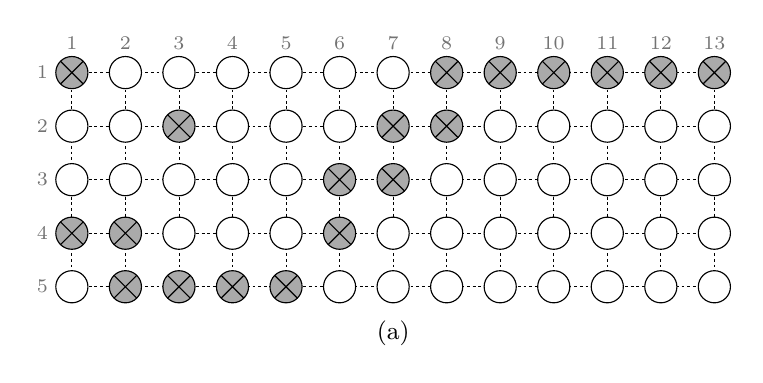
\begin{tikzpicture}[x=0.68cm,y=0.68cm,baseline=(current bounding box.north)]
  \begin{scope}[xshift=0.000cm]
    \draw[black,line width=0.27pt,dash pattern=on 1.02pt off 1.02pt] (1,-1) -- (13,-1) (1,-2) -- (13,-2) (1,-3) -- (13,-3) (1,-4) -- (13,-4) (1,-5) -- (13,-5) (1,-1) -- (1,-5) (2,-1) -- (2,-5) (3,-1) -- (3,-5) (4,-1) -- (4,-5) (5,-1) -- (5,-5) (6,-1) -- (6,-5) (7,-1) -- (7,-5) (8,-1) -- (8,-5) (9,-1) -- (9,-5) (10,-1) -- (10,-5) (11,-1) -- (11,-5) (12,-1) -- (12,-5) (13,-1) -- (13,-5);
    \filldraw[fill=kgray,draw=black,line width=0.41pt] (1,-1) circle (0.3);
    \draw[black,line width=0.41pt] (0.788,-0.788) -- (1.212,-1.212) (0.788,-1.212) -- (1.212,-0.788);
    \filldraw[fill=white,draw=black,line width=0.41pt] (2,-1) circle (0.3);
    \filldraw[fill=white,draw=black,line width=0.41pt] (3,-1) circle (0.3);
    \filldraw[fill=white,draw=black,line width=0.41pt] (4,-1) circle (0.3);
    \filldraw[fill=white,draw=black,line width=0.41pt] (5,-1) circle (0.3);
    \filldraw[fill=white,draw=black,line width=0.41pt] (6,-1) circle (0.3);
    \filldraw[fill=white,draw=black,line width=0.41pt] (7,-1) circle (0.3);
    \filldraw[fill=kgray,draw=black,line width=0.41pt] (8,-1) circle (0.3);
    \draw[black,line width=0.41pt] (7.788,-0.788) -- (8.212,-1.212) (7.788,-1.212) -- (8.212,-0.788);
    \filldraw[fill=kgray,draw=black,line width=0.41pt] (9,-1) circle (0.3);
    \draw[black,line width=0.41pt] (8.788,-0.788) -- (9.212,-1.212) (8.788,-1.212) -- (9.212,-0.788);
    \filldraw[fill=kgray,draw=black,line width=0.41pt] (10,-1) circle (0.3);
    \draw[black,line width=0.41pt] (9.788,-0.788) -- (10.212,-1.212) (9.788,-1.212) -- (10.212,-0.788);
    \filldraw[fill=kgray,draw=black,line width=0.41pt] (11,-1) circle (0.3);
    \draw[black,line width=0.41pt] (10.788,-0.788) -- (11.212,-1.212) (10.788,-1.212) -- (11.212,-0.788);
    \filldraw[fill=kgray,draw=black,line width=0.41pt] (12,-1) circle (0.3);
    \draw[black,line width=0.41pt] (11.788,-0.788) -- (12.212,-1.212) (11.788,-1.212) -- (12.212,-0.788);
    \filldraw[fill=kgray,draw=black,line width=0.41pt] (13,-1) circle (0.3);
    \draw[black,line width=0.41pt] (12.788,-0.788) -- (13.212,-1.212) (12.788,-1.212) -- (13.212,-0.788);
    \filldraw[fill=white,draw=black,line width=0.41pt] (1,-2) circle (0.3);
    \filldraw[fill=white,draw=black,line width=0.41pt] (2,-2) circle (0.3);
    \filldraw[fill=kgray,draw=black,line width=0.41pt] (3,-2) circle (0.3);
    \draw[black,line width=0.41pt] (2.788,-1.788) -- (3.212,-2.212) (2.788,-2.212) -- (3.212,-1.788);
    \filldraw[fill=white,draw=black,line width=0.41pt] (4,-2) circle (0.3);
    \filldraw[fill=white,draw=black,line width=0.41pt] (5,-2) circle (0.3);
    \filldraw[fill=white,draw=black,line width=0.41pt] (6,-2) circle (0.3);
    \filldraw[fill=kgray,draw=black,line width=0.41pt] (7,-2) circle (0.3);
    \draw[black,line width=0.41pt] (6.788,-1.788) -- (7.212,-2.212) (6.788,-2.212) -- (7.212,-1.788);
    \filldraw[fill=kgray,draw=black,line width=0.41pt] (8,-2) circle (0.3);
    \draw[black,line width=0.41pt] (7.788,-1.788) -- (8.212,-2.212) (7.788,-2.212) -- (8.212,-1.788);
    \filldraw[fill=white,draw=black,line width=0.41pt] (9,-2) circle (0.3);
    \filldraw[fill=white,draw=black,line width=0.41pt] (10,-2) circle (0.3);
    \filldraw[fill=white,draw=black,line width=0.41pt] (11,-2) circle (0.3);
    \filldraw[fill=white,draw=black,line width=0.41pt] (12,-2) circle (0.3);
    \filldraw[fill=white,draw=black,line width=0.41pt] (13,-2) circle (0.3);
    \filldraw[fill=white,draw=black,line width=0.41pt] (1,-3) circle (0.3);
    \filldraw[fill=white,draw=black,line width=0.41pt] (2,-3) circle (0.3);
    \filldraw[fill=white,draw=black,line width=0.41pt] (3,-3) circle (0.3);
    \filldraw[fill=white,draw=black,line width=0.41pt] (4,-3) circle (0.3);
    \filldraw[fill=white,draw=black,line width=0.41pt] (5,-3) circle (0.3);
    \filldraw[fill=kgray,draw=black,line width=0.41pt] (6,-3) circle (0.3);
    \draw[black,line width=0.41pt] (5.788,-2.788) -- (6.212,-3.212) (5.788,-3.212) -- (6.212,-2.788);
    \filldraw[fill=kgray,draw=black,line width=0.41pt] (7,-3) circle (0.3);
    \draw[black,line width=0.41pt] (6.788,-2.788) -- (7.212,-3.212) (6.788,-3.212) -- (7.212,-2.788);
    \filldraw[fill=white,draw=black,line width=0.41pt] (8,-3) circle (0.3);
    \filldraw[fill=white,draw=black,line width=0.41pt] (9,-3) circle (0.3);
    \filldraw[fill=white,draw=black,line width=0.41pt] (10,-3) circle (0.3);
    \filldraw[fill=white,draw=black,line width=0.41pt] (11,-3) circle (0.3);
    \filldraw[fill=white,draw=black,line width=0.41pt] (12,-3) circle (0.3);
    \filldraw[fill=white,draw=black,line width=0.41pt] (13,-3) circle (0.3);
    \filldraw[fill=kgray,draw=black,line width=0.41pt] (1,-4) circle (0.3);
    \draw[black,line width=0.41pt] (0.788,-3.788) -- (1.212,-4.212) (0.788,-4.212) -- (1.212,-3.788);
    \filldraw[fill=kgray,draw=black,line width=0.41pt] (2,-4) circle (0.3);
    \draw[black,line width=0.41pt] (1.788,-3.788) -- (2.212,-4.212) (1.788,-4.212) -- (2.212,-3.788);
    \filldraw[fill=white,draw=black,line width=0.41pt] (3,-4) circle (0.3);
    \filldraw[fill=white,draw=black,line width=0.41pt] (4,-4) circle (0.3);
    \filldraw[fill=white,draw=black,line width=0.41pt] (5,-4) circle (0.3);
    \filldraw[fill=kgray,draw=black,line width=0.41pt] (6,-4) circle (0.3);
    \draw[black,line width=0.41pt] (5.788,-3.788) -- (6.212,-4.212) (5.788,-4.212) -- (6.212,-3.788);
    \filldraw[fill=white,draw=black,line width=0.41pt] (7,-4) circle (0.3);
    \filldraw[fill=white,draw=black,line width=0.41pt] (8,-4) circle (0.3);
    \filldraw[fill=white,draw=black,line width=0.41pt] (9,-4) circle (0.3);
    \filldraw[fill=white,draw=black,line width=0.41pt] (10,-4) circle (0.3);
    \filldraw[fill=white,draw=black,line width=0.41pt] (11,-4) circle (0.3);
    \filldraw[fill=white,draw=black,line width=0.41pt] (12,-4) circle (0.3);
    \filldraw[fill=white,draw=black,line width=0.41pt] (13,-4) circle (0.3);
    \filldraw[fill=white,draw=black,line width=0.41pt] (1,-5) circle (0.3);
    \filldraw[fill=kgray,draw=black,line width=0.41pt] (2,-5) circle (0.3);
    \draw[black,line width=0.41pt] (1.788,-4.788) -- (2.212,-5.212) (1.788,-5.212) -- (2.212,-4.788);
    \filldraw[fill=kgray,draw=black,line width=0.41pt] (3,-5) circle (0.3);
    \draw[black,line width=0.41pt] (2.788,-4.788) -- (3.212,-5.212) (2.788,-5.212) -- (3.212,-4.788);
    \filldraw[fill=kgray,draw=black,line width=0.41pt] (4,-5) circle (0.3);
    \draw[black,line width=0.41pt] (3.788,-4.788) -- (4.212,-5.212) (3.788,-5.212) -- (4.212,-4.788);
    \filldraw[fill=kgray,draw=black,line width=0.41pt] (5,-5) circle (0.3);
    \draw[black,line width=0.41pt] (4.788,-4.788) -- (5.212,-5.212) (4.788,-5.212) -- (5.212,-4.788);
    \filldraw[fill=white,draw=black,line width=0.41pt] (6,-5) circle (0.3);
    \filldraw[fill=white,draw=black,line width=0.41pt] (7,-5) circle (0.3);
    \filldraw[fill=white,draw=black,line width=0.41pt] (8,-5) circle (0.3);
    \filldraw[fill=white,draw=black,line width=0.41pt] (9,-5) circle (0.3);
    \filldraw[fill=white,draw=black,line width=0.41pt] (10,-5) circle (0.3);
    \filldraw[fill=white,draw=black,line width=0.41pt] (11,-5) circle (0.3);
    \filldraw[fill=white,draw=black,line width=0.41pt] (12,-5) circle (0.3);
    \filldraw[fill=white,draw=black,line width=0.41pt] (13,-5) circle (0.3);
    \node[lab] at (1,-0.45) {1};
    \node[lab] at (2,-0.45) {2};
    \node[lab] at (3,-0.45) {3};
    \node[lab] at (4,-0.45) {4};
    \node[lab] at (5,-0.45) {5};
    \node[lab] at (6,-0.45) {6};
    \node[lab] at (7,-0.45) {7};
    \node[lab] at (8,-0.45) {8};
    \node[lab] at (9,-0.45) {9};
    \node[lab] at (10,-0.45) {10};
    \node[lab] at (11,-0.45) {11};
    \node[lab] at (12,-0.45) {12};
    \node[lab] at (13,-0.45) {13};
    \node[lab] at (0.45,-1) {1};
    \node[lab] at (0.45,-2) {2};
    \node[lab] at (0.45,-3) {3};
    \node[lab] at (0.45,-4) {4};
    \node[lab] at (0.45,-5) {5};
    \node[capt,anchor=north] at (7.00,-5.45) {(a)};
  \end{scope}
\end{tikzpicture}

\par\medskip
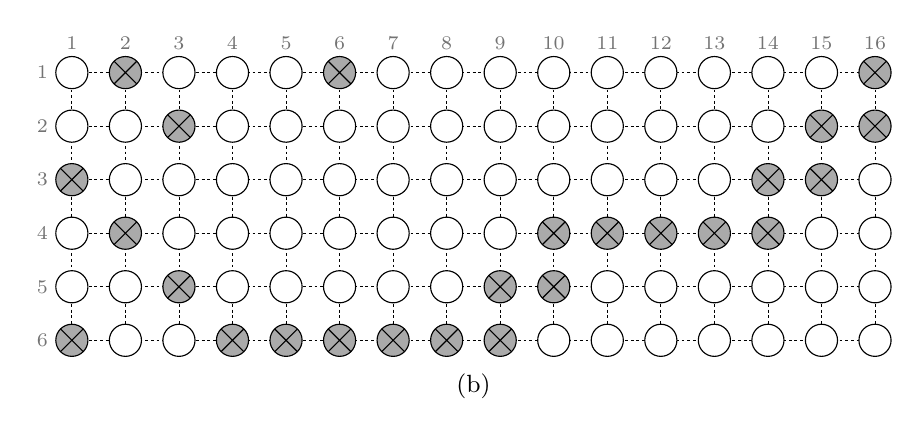
\begin{tikzpicture}[x=0.68cm,y=0.68cm,baseline=(current bounding box.north)]
  \begin{scope}[xshift=0.000cm]
    \draw[black,line width=0.27pt,dash pattern=on 1.02pt off 1.02pt] (1,-1) -- (16,-1) (1,-2) -- (16,-2) (1,-3) -- (16,-3) (1,-4) -- (16,-4) (1,-5) -- (16,-5) (1,-6) -- (16,-6) (1,-1) -- (1,-6) (2,-1) -- (2,-6) (3,-1) -- (3,-6) (4,-1) -- (4,-6) (5,-1) -- (5,-6) (6,-1) -- (6,-6) (7,-1) -- (7,-6) (8,-1) -- (8,-6) (9,-1) -- (9,-6) (10,-1) -- (10,-6) (11,-1) -- (11,-6) (12,-1) -- (12,-6) (13,-1) -- (13,-6) (14,-1) -- (14,-6) (15,-1) -- (15,-6) (16,-1) -- (16,-6);
    \filldraw[fill=white,draw=black,line width=0.41pt] (1,-1) circle (0.3);
    \filldraw[fill=kgray,draw=black,line width=0.41pt] (2,-1) circle (0.3);
    \draw[black,line width=0.41pt] (1.788,-0.788) -- (2.212,-1.212) (1.788,-1.212) -- (2.212,-0.788);
    \filldraw[fill=white,draw=black,line width=0.41pt] (3,-1) circle (0.3);
    \filldraw[fill=white,draw=black,line width=0.41pt] (4,-1) circle (0.3);
    \filldraw[fill=white,draw=black,line width=0.41pt] (5,-1) circle (0.3);
    \filldraw[fill=kgray,draw=black,line width=0.41pt] (6,-1) circle (0.3);
    \draw[black,line width=0.41pt] (5.788,-0.788) -- (6.212,-1.212) (5.788,-1.212) -- (6.212,-0.788);
    \filldraw[fill=white,draw=black,line width=0.41pt] (7,-1) circle (0.3);
    \filldraw[fill=white,draw=black,line width=0.41pt] (8,-1) circle (0.3);
    \filldraw[fill=white,draw=black,line width=0.41pt] (9,-1) circle (0.3);
    \filldraw[fill=white,draw=black,line width=0.41pt] (10,-1) circle (0.3);
    \filldraw[fill=white,draw=black,line width=0.41pt] (11,-1) circle (0.3);
    \filldraw[fill=white,draw=black,line width=0.41pt] (12,-1) circle (0.3);
    \filldraw[fill=white,draw=black,line width=0.41pt] (13,-1) circle (0.3);
    \filldraw[fill=white,draw=black,line width=0.41pt] (14,-1) circle (0.3);
    \filldraw[fill=white,draw=black,line width=0.41pt] (15,-1) circle (0.3);
    \filldraw[fill=kgray,draw=black,line width=0.41pt] (16,-1) circle (0.3);
    \draw[black,line width=0.41pt] (15.788,-0.788) -- (16.212,-1.212) (15.788,-1.212) -- (16.212,-0.788);
    \filldraw[fill=white,draw=black,line width=0.41pt] (1,-2) circle (0.3);
    \filldraw[fill=white,draw=black,line width=0.41pt] (2,-2) circle (0.3);
    \filldraw[fill=kgray,draw=black,line width=0.41pt] (3,-2) circle (0.3);
    \draw[black,line width=0.41pt] (2.788,-1.788) -- (3.212,-2.212) (2.788,-2.212) -- (3.212,-1.788);
    \filldraw[fill=white,draw=black,line width=0.41pt] (4,-2) circle (0.3);
    \filldraw[fill=white,draw=black,line width=0.41pt] (5,-2) circle (0.3);
    \filldraw[fill=white,draw=black,line width=0.41pt] (6,-2) circle (0.3);
    \filldraw[fill=white,draw=black,line width=0.41pt] (7,-2) circle (0.3);
    \filldraw[fill=white,draw=black,line width=0.41pt] (8,-2) circle (0.3);
    \filldraw[fill=white,draw=black,line width=0.41pt] (9,-2) circle (0.3);
    \filldraw[fill=white,draw=black,line width=0.41pt] (10,-2) circle (0.3);
    \filldraw[fill=white,draw=black,line width=0.41pt] (11,-2) circle (0.3);
    \filldraw[fill=white,draw=black,line width=0.41pt] (12,-2) circle (0.3);
    \filldraw[fill=white,draw=black,line width=0.41pt] (13,-2) circle (0.3);
    \filldraw[fill=white,draw=black,line width=0.41pt] (14,-2) circle (0.3);
    \filldraw[fill=kgray,draw=black,line width=0.41pt] (15,-2) circle (0.3);
    \draw[black,line width=0.41pt] (14.788,-1.788) -- (15.212,-2.212) (14.788,-2.212) -- (15.212,-1.788);
    \filldraw[fill=kgray,draw=black,line width=0.41pt] (16,-2) circle (0.3);
    \draw[black,line width=0.41pt] (15.788,-1.788) -- (16.212,-2.212) (15.788,-2.212) -- (16.212,-1.788);
    \filldraw[fill=kgray,draw=black,line width=0.41pt] (1,-3) circle (0.3);
    \draw[black,line width=0.41pt] (0.788,-2.788) -- (1.212,-3.212) (0.788,-3.212) -- (1.212,-2.788);
    \filldraw[fill=white,draw=black,line width=0.41pt] (2,-3) circle (0.3);
    \filldraw[fill=white,draw=black,line width=0.41pt] (3,-3) circle (0.3);
    \filldraw[fill=white,draw=black,line width=0.41pt] (4,-3) circle (0.3);
    \filldraw[fill=white,draw=black,line width=0.41pt] (5,-3) circle (0.3);
    \filldraw[fill=white,draw=black,line width=0.41pt] (6,-3) circle (0.3);
    \filldraw[fill=white,draw=black,line width=0.41pt] (7,-3) circle (0.3);
    \filldraw[fill=white,draw=black,line width=0.41pt] (8,-3) circle (0.3);
    \filldraw[fill=white,draw=black,line width=0.41pt] (9,-3) circle (0.3);
    \filldraw[fill=white,draw=black,line width=0.41pt] (10,-3) circle (0.3);
    \filldraw[fill=white,draw=black,line width=0.41pt] (11,-3) circle (0.3);
    \filldraw[fill=white,draw=black,line width=0.41pt] (12,-3) circle (0.3);
    \filldraw[fill=white,draw=black,line width=0.41pt] (13,-3) circle (0.3);
    \filldraw[fill=kgray,draw=black,line width=0.41pt] (14,-3) circle (0.3);
    \draw[black,line width=0.41pt] (13.788,-2.788) -- (14.212,-3.212) (13.788,-3.212) -- (14.212,-2.788);
    \filldraw[fill=kgray,draw=black,line width=0.41pt] (15,-3) circle (0.3);
    \draw[black,line width=0.41pt] (14.788,-2.788) -- (15.212,-3.212) (14.788,-3.212) -- (15.212,-2.788);
    \filldraw[fill=white,draw=black,line width=0.41pt] (16,-3) circle (0.3);
    \filldraw[fill=white,draw=black,line width=0.41pt] (1,-4) circle (0.3);
    \filldraw[fill=kgray,draw=black,line width=0.41pt] (2,-4) circle (0.3);
    \draw[black,line width=0.41pt] (1.788,-3.788) -- (2.212,-4.212) (1.788,-4.212) -- (2.212,-3.788);
    \filldraw[fill=white,draw=black,line width=0.41pt] (3,-4) circle (0.3);
    \filldraw[fill=white,draw=black,line width=0.41pt] (4,-4) circle (0.3);
    \filldraw[fill=white,draw=black,line width=0.41pt] (5,-4) circle (0.3);
    \filldraw[fill=white,draw=black,line width=0.41pt] (6,-4) circle (0.3);
    \filldraw[fill=white,draw=black,line width=0.41pt] (7,-4) circle (0.3);
    \filldraw[fill=white,draw=black,line width=0.41pt] (8,-4) circle (0.3);
    \filldraw[fill=white,draw=black,line width=0.41pt] (9,-4) circle (0.3);
    \filldraw[fill=kgray,draw=black,line width=0.41pt] (10,-4) circle (0.3);
    \draw[black,line width=0.41pt] (9.788,-3.788) -- (10.212,-4.212) (9.788,-4.212) -- (10.212,-3.788);
    \filldraw[fill=kgray,draw=black,line width=0.41pt] (11,-4) circle (0.3);
    \draw[black,line width=0.41pt] (10.788,-3.788) -- (11.212,-4.212) (10.788,-4.212) -- (11.212,-3.788);
    \filldraw[fill=kgray,draw=black,line width=0.41pt] (12,-4) circle (0.3);
    \draw[black,line width=0.41pt] (11.788,-3.788) -- (12.212,-4.212) (11.788,-4.212) -- (12.212,-3.788);
    \filldraw[fill=kgray,draw=black,line width=0.41pt] (13,-4) circle (0.3);
    \draw[black,line width=0.41pt] (12.788,-3.788) -- (13.212,-4.212) (12.788,-4.212) -- (13.212,-3.788);
    \filldraw[fill=kgray,draw=black,line width=0.41pt] (14,-4) circle (0.3);
    \draw[black,line width=0.41pt] (13.788,-3.788) -- (14.212,-4.212) (13.788,-4.212) -- (14.212,-3.788);
    \filldraw[fill=white,draw=black,line width=0.41pt] (15,-4) circle (0.3);
    \filldraw[fill=white,draw=black,line width=0.41pt] (16,-4) circle (0.3);
    \filldraw[fill=white,draw=black,line width=0.41pt] (1,-5) circle (0.3);
    \filldraw[fill=white,draw=black,line width=0.41pt] (2,-5) circle (0.3);
    \filldraw[fill=kgray,draw=black,line width=0.41pt] (3,-5) circle (0.3);
    \draw[black,line width=0.41pt] (2.788,-4.788) -- (3.212,-5.212) (2.788,-5.212) -- (3.212,-4.788);
    \filldraw[fill=white,draw=black,line width=0.41pt] (4,-5) circle (0.3);
    \filldraw[fill=white,draw=black,line width=0.41pt] (5,-5) circle (0.3);
    \filldraw[fill=white,draw=black,line width=0.41pt] (6,-5) circle (0.3);
    \filldraw[fill=white,draw=black,line width=0.41pt] (7,-5) circle (0.3);
    \filldraw[fill=white,draw=black,line width=0.41pt] (8,-5) circle (0.3);
    \filldraw[fill=kgray,draw=black,line width=0.41pt] (9,-5) circle (0.3);
    \draw[black,line width=0.41pt] (8.788,-4.788) -- (9.212,-5.212) (8.788,-5.212) -- (9.212,-4.788);
    \filldraw[fill=kgray,draw=black,line width=0.41pt] (10,-5) circle (0.3);
    \draw[black,line width=0.41pt] (9.788,-4.788) -- (10.212,-5.212) (9.788,-5.212) -- (10.212,-4.788);
    \filldraw[fill=white,draw=black,line width=0.41pt] (11,-5) circle (0.3);
    \filldraw[fill=white,draw=black,line width=0.41pt] (12,-5) circle (0.3);
    \filldraw[fill=white,draw=black,line width=0.41pt] (13,-5) circle (0.3);
    \filldraw[fill=white,draw=black,line width=0.41pt] (14,-5) circle (0.3);
    \filldraw[fill=white,draw=black,line width=0.41pt] (15,-5) circle (0.3);
    \filldraw[fill=white,draw=black,line width=0.41pt] (16,-5) circle (0.3);
    \filldraw[fill=kgray,draw=black,line width=0.41pt] (1,-6) circle (0.3);
    \draw[black,line width=0.41pt] (0.788,-5.788) -- (1.212,-6.212) (0.788,-6.212) -- (1.212,-5.788);
    \filldraw[fill=white,draw=black,line width=0.41pt] (2,-6) circle (0.3);
    \filldraw[fill=white,draw=black,line width=0.41pt] (3,-6) circle (0.3);
    \filldraw[fill=kgray,draw=black,line width=0.41pt] (4,-6) circle (0.3);
    \draw[black,line width=0.41pt] (3.788,-5.788) -- (4.212,-6.212) (3.788,-6.212) -- (4.212,-5.788);
    \filldraw[fill=kgray,draw=black,line width=0.41pt] (5,-6) circle (0.3);
    \draw[black,line width=0.41pt] (4.788,-5.788) -- (5.212,-6.212) (4.788,-6.212) -- (5.212,-5.788);
    \filldraw[fill=kgray,draw=black,line width=0.41pt] (6,-6) circle (0.3);
    \draw[black,line width=0.41pt] (5.788,-5.788) -- (6.212,-6.212) (5.788,-6.212) -- (6.212,-5.788);
    \filldraw[fill=kgray,draw=black,line width=0.41pt] (7,-6) circle (0.3);
    \draw[black,line width=0.41pt] (6.788,-5.788) -- (7.212,-6.212) (6.788,-6.212) -- (7.212,-5.788);
    \filldraw[fill=kgray,draw=black,line width=0.41pt] (8,-6) circle (0.3);
    \draw[black,line width=0.41pt] (7.788,-5.788) -- (8.212,-6.212) (7.788,-6.212) -- (8.212,-5.788);
    \filldraw[fill=kgray,draw=black,line width=0.41pt] (9,-6) circle (0.3);
    \draw[black,line width=0.41pt] (8.788,-5.788) -- (9.212,-6.212) (8.788,-6.212) -- (9.212,-5.788);
    \filldraw[fill=white,draw=black,line width=0.41pt] (10,-6) circle (0.3);
    \filldraw[fill=white,draw=black,line width=0.41pt] (11,-6) circle (0.3);
    \filldraw[fill=white,draw=black,line width=0.41pt] (12,-6) circle (0.3);
    \filldraw[fill=white,draw=black,line width=0.41pt] (13,-6) circle (0.3);
    \filldraw[fill=white,draw=black,line width=0.41pt] (14,-6) circle (0.3);
    \filldraw[fill=white,draw=black,line width=0.41pt] (15,-6) circle (0.3);
    \filldraw[fill=white,draw=black,line width=0.41pt] (16,-6) circle (0.3);
    \node[lab] at (1,-0.45) {1};
    \node[lab] at (2,-0.45) {2};
    \node[lab] at (3,-0.45) {3};
    \node[lab] at (4,-0.45) {4};
    \node[lab] at (5,-0.45) {5};
    \node[lab] at (6,-0.45) {6};
    \node[lab] at (7,-0.45) {7};
    \node[lab] at (8,-0.45) {8};
    \node[lab] at (9,-0.45) {9};
    \node[lab] at (10,-0.45) {10};
    \node[lab] at (11,-0.45) {11};
    \node[lab] at (12,-0.45) {12};
    \node[lab] at (13,-0.45) {13};
    \node[lab] at (14,-0.45) {14};
    \node[lab] at (15,-0.45) {15};
    \node[lab] at (16,-0.45) {16};
    \node[lab] at (0.45,-1) {1};
    \node[lab] at (0.45,-2) {2};
    \node[lab] at (0.45,-3) {3};
    \node[lab] at (0.45,-4) {4};
    \node[lab] at (0.45,-5) {5};
    \node[lab] at (0.45,-6) {6};
    \node[capt,anchor=north] at (8.50,-6.45) {(b)};
  \end{scope}
\end{tikzpicture}

\caption{(a) The $5\times13$ test board of $S_8$. (b) The $6\times16$ blackout $S_{16}$.}
\label{fig:boards}
\end{figure}

\begin{theorem}[five rows, (a) and (c) computer-assisted, (b) checked in Lean]\label{thm:fiverow}
\leavevmode
\begin{enumerate}[(a)]
\item We have $f(5,m)=m+5$ for $m=5$, $6$, and $7$.
\item We have $f(5,m)=m+6$ for every $m\ge8$, attained by $S_8$ followed by $m-8$ columns black in
row $1$ only.
\item The $5\times8$ grid has exactly four maximum blackouts, the images of $S_8$ under row
reflection and column reversal.
\end{enumerate}
\end{theorem}

\begin{proof}
(b) The upper bound is Theorem~\ref{thm:rowbound}.
For the construction, $W_5=5$, so the collar theorem with right padding
in row $1$ reduces the whole family from $S_8$ to Figure~\ref{fig:boards}(a).
Three enumerators and Lean verify that the $954$ rectangles of this
test board have different presentations.
(a) At $m=5$, use Corollary~\ref{cor:small-m} and the construction $S_0$
in Theorem~\ref{thm:fivefive}. At $m=6,7$, the constructions are
$15,\allowbreak 12,\allowbreak 23,\allowbreak 3,\allowbreak 34,\allowbreak 45$ and
$1,\allowbreak 12,\allowbreak 23,\allowbreak 3,\allowbreak 34,\allowbreak 45,\allowbreak 15$,
recorded in \nolinkurl{jis/data/small_cells_sat_5x6.json} and
\nolinkurl{jis/data/small_cells_sat_5x7_b12.json}. They give the lower
bounds. Checked SAT certificates rule out $m+6$ points
(Section~\ref{sec:verify}).
(c) Two SAT enumerations find the four images. A separate column search
checks all $10\,(8)_6\,5^2=5{,}040{,}000$ equality candidates from
Theorem~\ref{thm:equality} and finds the same four.
\end{proof}

Theorem~\ref{thm:A} gives $f(h,m)\le h+m$ whenever a side is at most
four, and on $5\times5$, $5\times6$, $5\times7$, and $6\times6$.
Up to transposition, these exhaust the grids of area below $40$.
Thus $5\times8$ is the first failure of the guess $f(h,m)=h+m$.

\begin{remark}[five-row counts, computer-assisted]\label{rem:fivecounts}
The counts $a_5(m)$ for $8\le m\le23$ are \seqnum{A401225}. They begin $4$, $44$, $350$,
$3{,}004$, $24{,}706$, and $193{,}406$, and $a_5(23)=5{,}510{,}071{,}794{,}736$. For $m\ge13$
each count agrees in two independent transfer calculations using the equality structure of
Theorem~\ref{thm:equality}.
\end{remark}

\subsection{Six rows and small grids}

Let $S_{16}$ be the blackout of the $6\times16$ grid in Figure~\ref{fig:boards}(b). Its doubles,
in the columns $1,2,3,6,9,10,14,15,16$, carry the edges of $K_{3,3}$ between $\{1,3,5\}$ and
$\{2,4,6\}$.

One point below the row bound, the structure is still rigid.

\begin{lemma}[one point below the bound]\label{lem:sixbelow}
Let $m\ge3$, and let $S$ be an axis-valid blackout of the $6\times m$ grid with $m+8$ points.
Then every column of $S$ is empty, a singleton, or a double, the doubles have distinct row
pairs, and one of the following holds.
\begin{enumerate}[(a)]
\item No column is empty, and the pairs of the doubles are the edges of $K_{3,3}$ minus one edge.
\item No column is empty, and the pairs of the doubles are the edges of $K_{2,4}$.
\item Exactly one column is empty, and the pairs of the doubles are the edges of $K_{3,3}$.
\end{enumerate}
\end{lemma}

\begin{proof}
By Lemma~\ref{lem:H}, $|S|=t+e(H)$ for every choice of the trees, where $t\le m$ counts the
nonempty columns. Mantel gives $e(H)\le9$ (Lemma~\ref{lem:mantel}), so $(t,e(H))$ is $(m,8)$ or
$(m-1,9)$.

In the second case $H$ has $q_6$ edges. The proof of Theorem~\ref{thm:equality} then shows
that $H$ is $K_{3,3}$ and that no column has three black rows, which gives (c).

In the first case $H$ is triangle-free with $8$ edges. Suppose $H$ is not bipartite. Then its
shortest odd cycle is a five-cycle, which has no chord. The sixth vertex is adjacent to at most
two of its vertices, so $e(H)\le7$, a contradiction. Hence $H$ is bipartite with parts of sizes
$k$ and $6-k$, and $k(6-k)\ge8$ forces $H$ to be $K_{2,4}$ or $K_{3,3}$ minus an edge. In both
graphs, two vertices in the same part have at least two common neighbors.
Now suppose $|B_i|\ge3$. Then $T_i$ has a vertex $v$ with two neighbors $u$ and $w$. These lie
in the same part of $H$, so they have a common neighbor $z\ne v$. Replacing the edge $vw$ of
$T_i$ by $uw$ gives another tree on $B_i$, and the new graph $H$ contains the triangle $uwz$.
This contradicts Lemma~\ref{lem:H}. Thus every column is a singleton or a double, and the
pairs of the doubles are the edges of $H$. They are distinct because $H$ is simple.
\end{proof}

There are $10\cdot9=90$ labeled graphs in case (a), $15$ in case (b), and $10$ in case (c).

\begin{theorem}[six rows, (a) and (b) computer-assisted, (c) checked in Lean]\label{thm:sixrow}
\leavevmode
\begin{enumerate}[(a)]
\item For $8\le m\le11$ we have $f(6,m)=m+7$.
\item For $12\le m\le14$ we have $f(6,m)=m+8$, attained by the blackout
$16,\allowbreak 36,\allowbreak 25,\allowbreak 12,\allowbreak 1^{m-8},\allowbreak 23,\allowbreak 34,\allowbreak 45,\allowbreak 56$, where $1^{k}$ denotes $k$
columns black only in row $1$.
\item For every $m\ge15$ we have $f(6,m)=m+9$.
\end{enumerate}
So $f(h,m)$ is known for every $h\le6$ and every $m$.
\end{theorem}

\begin{proof}
For $9\le m\le14$, an optimum with $m+9$ points would have double
columns carrying $K_{3,3}$, by Theorem~\ref{thm:equality}.
There are ten possible row partitions. The structured encoding has
checked LRAT certificates excluding every one (Lemma~\ref{lem:enc}).
At $m=8$, Corollary~\ref{cor:small-m} gives the same bound.
Hence $f(6,m)\le m+8$ for $8\le m\le14$.

(a) The case $m=8$ is Theorem~\ref{thm:refute}. For the lower bound at $9\le m\le11$, the
blackout $12,\allowbreak 23,\allowbreak 34,\allowbreak 45,\allowbreak 6,\allowbreak 6,\allowbreak 36,\allowbreak 56,\allowbreak 25$ of the $6\times9$ grid is valid with $16$ points. Its
collar test board, with $W_6=7$ columns black only in row $1$ on each side, is valid
(\nolinkurl{six_row_collar_6x9_check.py}), so Theorem~\ref{thm:collar} gives $m+7$ points at every
$m\ge9$. For the upper bound, Lemma~\ref{lem:sixbelow} leaves $115$ structured instances at each
width, one for each labeled graph in its three cases. They are unsatisfiable under two
encodings, and encoding A has checked LRAT certificates.

(b) Three enumerators check that the blackout is valid. It has $m+8$ points.

(c) Again the row bound gives the upper bound. For $m=15$, take
$56,\allowbreak 45,\allowbreak 34,\allowbreak 23,\allowbreak 1,\allowbreak 1,\allowbreak 14,\allowbreak 1,\allowbreak 1,\allowbreak 12,\allowbreak 36,\allowbreak 1,\allowbreak 25,\allowbreak 6,\allowbreak 16$
from \nolinkurl{jis/data/six_row_sat_w15_A.json}, which is valid with
$24$ points. For $m\ge16$, apply the collar theorem to $S_{16}$ in
Figure~\ref{fig:boards}(b). Since $W_6=7$, it suffices to add
$(17,1),\dots,(23,1)$. Three enumerators and Lean verify distinct
presentations for all $4{,}627$ rectangles of that test board.
\end{proof}

\begin{theorem}[seven rows, computer-assisted]\label{thm:sevenrow}
For every $m\ge24$ we have $f(7,m)=m+12$.
\end{theorem}

\begin{proof}
The row bound gives $f(7,m)\le m+12$. For the lower bounds we use the structured encoding A
of Section~\ref{sec:verify} with twelve doubles on the edges of $K_{3,4}$, for the partitions
of the rows into $\{2,4,6\}$ and $\{1,3,5,7\}$ (widths $24$, $25$, $26$, and $28$) and into
$\{1,4,7\}$ and $\{2,3,5,6\}$ (width $27$). It finds the valid blackouts
\begin{gather*}
56,45,34,23,1,1,14,1,12,1,6,16,7,1,47,6,67,7,7,6,25,7,36,27,\\
16,25,7,27,1,7,7,7,12,2,14,1,1,23,34,45,56,7,7,47,6,6,4,36,67,\\
67,47,23,12,1,7,1,2,2,25,5,36,6,6,45,1,6,27,1,1,1,7,34,14,56,16,\\
57,1,16,37,3,67,1,7,1,1,34,7,24,1,15,27,7,1,7,7,45,1,46,7,13,6,12,\\
34,2,2,2,47,2,2,27,25,7,7,7,7,7,67,36,23,2,12,1,1,16,1,1,14,1,45,56
\end{gather*}
of widths $24$ to $28$. Three enumerators confirm all five. The last one stays valid after adding
$W_7=10$ columns black only in row $7$ on its left. Theorem~\ref{thm:collar}, with padding
row $7$ on the left side, then gives $m+12$ points at every width $m\ge28$.
Three enumerators also confirm this collar test board.
\end{proof}

\begin{theorem}[small grids, computer-assisted]\label{thm:refute}
We have $f(6,6)=12$, $f(6,7)=13$, $f(7,7)=14$, and $f(6,8)=15$. The blackout
$15,\allowbreak 1,\allowbreak 123,\allowbreak 34,\allowbreak 4,\allowbreak 4,\allowbreak 456,\allowbreak 26$ of the $6\times8$ grid attains the last value.
\end{theorem}

\begin{proof}
The other constructions are $14,\allowbreak 1,\allowbreak 12,\allowbreak 2,\allowbreak 23,\allowbreak 3456$
on the $6\times6$ grid,
$16,\allowbreak 1,\allowbreak 1,\allowbreak 12,\allowbreak 2,\allowbreak 23,\allowbreak 3456$
on $6\times7$, and
$17,\allowbreak 1,\allowbreak 12,\allowbreak 2,\allowbreak 23,\allowbreak 3456,\allowbreak 67$
on $7\times7$. Their records are
\nolinkurl{jis/data/small_cells_sat_6x6.json},
\nolinkurl{jis/data/small_cells_sat_6x7.json}, and
\nolinkurl{jis/data/small_cells_sat_7x7.json}.
All are valid. For each grid, a checked SAT certificate excludes
one additional point.
\end{proof}

\begin{theorem}[the $5\times5$ grid]\label{thm:fivefive}
\leavevmode
\begin{enumerate}[(a)]
\item We have $f(5,5)=10$.
\item (Computer-assisted.) The $a_5(5)=8$ maximum blackouts are the images of $S_0$
below under the square's symmetries.
\end{enumerate}
\end{theorem}

\begin{proof}
(a) Corollary~\ref{cor:small-m} gives the upper bound. To attain it,
take $S_0$ to be $45,\allowbreak 34,\allowbreak 123,\allowbreak 1,\allowbreak 15$.
Its row-column graph is an $8$-cycle with two pendant edges, hence it is
axis-valid. Lemma~\ref{lem:leftmost} lists $30$ tilted rectangles, namely
nine unit diamonds, sixteen others from Lemma~\ref{lem:tilted-narrow},
and five spanning the grid. The fifteen weak rectangles show the pairs
below. After an oblique pair, the point following the bar is a white
corner of the axis-aligned rectangle through it.
\begin{center}\footnotesize
\begin{tabular}{@{}llll@{}}
$(1,2),(2,1)\mid(1,1)$ & $(1,3),(2,2)\mid(1,2)$ & $(3,4),(4,3)\mid(4,4)$ & $(2,5),(3,4)\mid(3,5)$ \\
$(2,2),(4,2)$ & $(1,2),(4,3)\mid(1,3)$ & $(4,4),(5,2)\mid(4,2)$ & $(3,5),(4,4)\mid(3,4)$ \\
$(4,3),(5,2)\mid(4,2)$ & $(3,4),(5,2)\mid(5,4)$ & $(2,5),(5,2)\mid(2,2)$ & $(4,5),(5,3)\mid(4,3)$ \\
$(1,3),(4,2)\mid(1,2)$ & $(2,5),(4,3)\mid(4,5)$ & & $(4,5),(5,4)\mid(4,4)$ \\
\end{tabular}
\end{center}
These pairs are all different. The other tilted rectangles show at least
three points, so Lemma~\ref{lem:threecorners} distinguishes them.
The listed white corners rule out axis-aligned rivals for every oblique
pair. The remaining pair $(2,2),(4,2)$ has no rival because
$B_2\cap B_4=\emptyset$. This proves validity.
(b) Three programs check all $44{,}640$ sets of $10$ points whose graph
has no four- or six-cycle. Only the images of $S_0$ are valid.
\end{proof}

\section{Every height at large widths}\label{sec:general}

The constructions of Sections~\ref{sec:four} and~\ref{sec:five} were found one height at a time.
For large widths a single pattern attains the row bound at every height. Call a singleton column
a \emph{sea} when its black point lies in row $1$ or in row $h$.

\begin{theorem}[large widths]\label{thm:general}
Let $h\ge3$ and put $M_h=q_h+(q_h-1)(2W_h+1)$. Then $f(h,m)=m+q_h$ for every $m\ge M_h$.
\end{theorem}

The upper bound is Theorem~\ref{thm:rowbound}. The lower bound follows from the next proposition,
which needs only a triangle-free graph on the rows.

\begin{proposition}[alternating seas]\label{prop:seas}
Let $h\ge3$ and let $H$ be a triangle-free graph on the rows with edges $e_1,\dots,e_q$.
Let $Z$ be the blackout of the $h\times m$ grid with doubles in columns $p_1<\dots<p_q$, where
column $p_j$ is black exactly in the two rows of $e_j$ and $p_{j+1}-p_j\ge2W_h+2$, and with a sea
in every other column. The seas to the left of $p_1$ are black in row $1$, and the row of the
seas switches between $1$ and $h$ at every double. Then $Z$ is valid and $|Z|=m+q$.
\end{proposition}

\begin{proof}[Proof of Theorem~\ref{thm:general}]
Take $H=K_{\lfloor h/2\rfloor,\lceil h/2\rceil}$, so $q=q_h$, and put the doubles in the columns
$p_j=1+(j-1)(2W_h+2)$. The last one is in column $1+(q_h-1)(2W_h+2)=M_h$, and every column
after it is a sea. Proposition~\ref{prop:seas} gives a valid blackout with $m+q_h$ points for
every $m\ge M_h$.
\end{proof}

In the proof of the proposition we use three facts about a tilted rectangle $R$ of the
$h\times m$ grid.
\begin{enumerate}[(F1)]
\item $R$ has at most one corner in row $1$ and at most one in row $h$. Indeed, a corner in row $1$
lies in the smallest row of $R$, which holds only one corner (Lemma~\ref{lem:leftmost}), and
likewise for row $h$.
\item A corner of $R$ in row $1$ and a corner in row $h$ are opposite. If they were adjacent, the
side joining them would be $(s,h-1)$, and the other two corners would be these two plus a nonzero
vector $n$ perpendicular to it. The corner in row $1$ needs $n_2\ge0$ and the corner in row $h$
needs $n_2\le0$, so $n_2=0$. Then $n_1s=0$ forces $s=0$, a vertical side, which is impossible.
\item Two corners of $R$ in one column are opposite, since a vertical side would make $R$
axis-aligned.
\end{enumerate}

\begin{proof}[Proof of Proposition~\ref{prop:seas}]
Each double adds one point to a column, so $|Z|=m+q$.

\emph{Axis-aligned rectangles.} Only doubles have two black rows, and their pairs are distinct,
so $G_Z$ has no four-cycle. A six-cycle $r_a\,c_x\,r_b\,c_y\,r_c\,c_z$ would need doubles on
$\{a,b\}$, $\{b,c\}$, and $\{a,c\}$, a triangle in $H$. By Lemma~\ref{lem:girth}, $Z$
distinguishes the axis-aligned rectangles, and none of them is hidden, since a hidden one would
give a four-cycle.

\emph{Locality.} A tilted rectangle $R$ has span at most $W_h$ (Lemma~\ref{lem:span}), so its
columns meet at most one double. If they meet none, all black points in these columns lie in one
boundary row, and $R$ has at most one black corner by (F1). Then $R$ shows at least three
corners. Otherwise we shift the columns so that the double is column $0$, with black rows
$a<b$. Reflecting the rows if necessary, which exchanges rows $1$ and $h$, we may assume that the
seas in the columns of $R$ are black in row $1$ to the left of column $0$ and in row $h$ to the
right of it.

Let $K$ be the set of black corners of $R$. By (F1), $K$ contains at most one point
$u=(x_1,1)$ with $x_1<0$, at most one point $v=(x_2,h)$ with $x_2>0$, and points $d=(0,c)$
with $c\in\{a,b\}$. A black corner $(0,1)$ or $(0,h)$ counts as a point $d$, and then (F1)
excludes $u$ or $v$, respectively. We consider $|K|\ge2$.

\begin{enumerate}[(a)]
\item $K=\{u,v\}$. These are opposite by (F2). The other diagonal has midpoint
$\mu=\bigl(\frac{x_1+x_2}2,\frac{1+h}2\bigr)$ and endpoints $\mu\pm w$ with
$|w|^2=\frac14\bigl((x_2-x_1)^2+(h-1)^2\bigr)$. By (F1) its endpoints lie in rows $2$ to $h-1$,
so $|w_2|\le\frac{h-3}2$ and $w_1^2>\frac14(x_2-x_1)^2$. Hence one endpoint lies in a column
smaller than $x_1$ and the other in a column larger than $x_2$. Neither is in column $0$, so both
are white.
\item $K=\{(0,a),(0,b)\}$. These are opposite by (F3). The other diagonal has midpoint
$\bigl(0,\frac{a+b}2\bigr)$, length $b-a$, and $w_1\ne0$, so $|w_2|<\frac{b-a}2$. Its endpoints
lie in the columns $\pm w_1$ and strictly between rows $a$ and $b$, so both are white.
\item $K=\{u,d\}$, opposite. Here $c\ge2$ by (F1). The other diagonal has midpoint
$\bigl(\frac{x_1}2,\frac{1+c}2\bigr)$ and $|w|^2=\frac14\bigl(x_1^2+(c-1)^2\bigr)$. Its endpoints
are not in row $1$ by (F1), not in row $h$ by (F2), since the opposite corner of $u$ is $d$, and
not in column $0$ by (F3). So both are white. Since their rows are at least $2$, we get
$|w_2|\le\frac{c-3}2$. Thus $c\ge3$ and $w_1^2>\frac14x_1^2$, so one endpoint lies in a column
larger than $0$ and the other in a column smaller than $x_1$.
\item $K=\{u,d\}$, adjacent. The side $d-u=(|x_1|,c-1)$ has $c\ge2$, and the other corners are
$u+n$ and $d+n$ with $n=t\bigl(-(c-1),|x_1|\bigr)$ for some $t\ne0$. The corner $u+n$ lies in row
$1+t|x_1|$, so $t>0$. Then both corners lie in negative columns and below row $1$, so both are
white. They differ by $(|x_1|,c-1)$, so they form an oblique pair.
\item $K$ contains $v$ and a point $d$ but not $u$. This is (c) or (d) after the half turn
$(x,j)\mapsto(-x,h+1-j)$, which exchanges the two seas and fixes column $0$.
\item $|K|\ge3$. If $K$ contains $(0,a)$ and $(0,b)$, the other two corners lie strictly between
rows $a$ and $b$ by (b), so they are neither $u$ nor $v$. Otherwise $K=\{u,d,v\}$. Then $u$ and
$v$ are opposite by (F2), and $d$ is adjacent to both, so $(u-d)\cdot(v-d)=0$, that is,
$x_1x_2=(c-1)(h-c)$. The left side is negative and the right side is not, a contradiction.
\end{enumerate}
Hence no tilted rectangle is hidden, and every weak tilted rectangle shows exactly two corners.
In (a) to (c) and their reflections, the shown corners lie in columns on both sides of column $0$.
In (d) and its reflection, they form an oblique pair on one side of column $0$.

\emph{Axis-aligned rivals.} By Lemma~\ref{lem:rival}, only a horizontal or an oblique pair needs
checking. A horizontal pair $\{(x,j),(z,j)\}$ arises only in (a) to (c), with $x<0<z$. There
$B_x=\{1\}$ and $B_z=\{h\}$ are disjoint, so it has no rival. For an oblique pair
$\{(x,j),(z,k)\}$, a rival needs $(x,k)$ and $(z,j)$ black. In (a) to (c), the rows $j,k$ lie
in $2,\dots,h-1$ and $x,z\ne0$, so these points are white. In (d), $x,z<0$ and $j,k\ge2$, so
again they are white.

\emph{Two tilted rectangles.} Let weak tilted rectangles $R\ne R'$ show the same pair $P$. The
columns of each contain $P$ and span at most $W_h$, so their doubles are at most $2W_h$ apart.
Hence they share the double in column $0$. If $P$ is a diagonal of both, their black diagonals
have the same midpoint and the same length. Comparing the cases, these determine the black
diagonal. For example, (a) against (c) forces $c=h$ from the midpoint rows, then $x_1'=x_1+x_2$
and $|x_1'|=x_2-x_1$, so $x_1=0$ or $x_2=0$. Case (b) has its midpoint in column $0$, and (a) can
match it only with $x_1=-x_2$ and $(2x_2)^2+(h-1)^2=(b-a)^2\le(h-1)^2$, which is impossible. The
other comparisons are similar or immediate. If $P$ is a side of exactly one of them, it lies on
one side of column $0$ by (d) and on both sides by (a) to (c), a contradiction.

Suppose finally that $P$ is a side of both, so the black sides $Y=P-n$ and $Y'=P-n'$ satisfy
$Y'=Y+(n-n')$. If both are of type (d), with $Y=\{u,d\}$ and $Y'=\{u',d'\}$, then matching $u$
with $u'$ gives $n=n'$, since $d,d'$ lie in column $0$ and $u,u'$ in row $1$. Matching $u$ with
$d'$ would put $u'$ in column $-x_1>0$. Two sides of the reflected type are symmetric. If
$Y=\{u,d\}$ and $Y'=\{d',v'\}$, matching $d$ with $d'$ would put $v'$ in column $x_1<0$. Matching
$u$ with $d'$ gives $n_1-n'_1=|x_1|>0$, but $n_1<0<n'_1$, since the other two corners of $R$ lie
to the left of column $0$ and those of $R'$ to the right. So $R=R'$.

Presentations of three or more points are unique (Lemma~\ref{lem:threecorners}), so $Z$ is
valid.
\end{proof}

By Theorem~\ref{thm:general}, $k_r=q_h$ for every residue in Theorem~\ref{thm:periodic}(a). The
threshold $M_h$ is far from the truth for small $h$. It is $61$ for $h=5$, while
$f(5,m)=m+6$ already from $m=8$, and the least widths for $h=4$, $5$, $6$, and $7$ are $6$, $8$,
$15$, and at most $24$.

\section{Every fixed height}\label{sec:height}

At fixed height $h$, finite memory suffices to test validity and count optima.
Read a blackout as the \emph{column word} $w=B_1\cdots B_m$, with $B_i$
recording column $i$'s black rows. Write $|w|=m$ and $S(w)$ for its blackout,
and let $\mathcal L_h$ be the valid words, including the empty word.
We first recognize all valid words, then add a bounded counter to select optima.

\begin{theorem}[regularity and rational series]\label{thm:regular}
For every $h\ge1$ the language $\mathcal L_h$ is regular, and $G_h(z,u)=\sum_{w\in\mathcal L_h}z^{|w|}u^{|S(w)|}$ is rational in $z$ and $u$.
\end{theorem}

\begin{proof}
The \emph{trace} of a rectangle records, in each column, the rows of its
corners. It determines the corner set. By Lemma~\ref{lem:diff}, two distinct
traces $Y,Y'$ give the same presentation exactly when
$Y_i\triangle Y'_i\subseteq B_i$ in every column.

The possible traces form a regular language. For an axis-aligned rectangle,
choose $r<s$, read a column $\{r,s\}$, then another such column after any
number of empty columns. There can also be empty columns before and after.
For a tilted rectangle, Lemmas~\ref{lem:leftmost} and~\ref{lem:span} leave
only finitely many templates~\eqref{eq:tilt-param}, each of span at most
$W_h$, again with arbitrary empty columns on either side.

An automaton can therefore read $w$ while guessing two rectangle traces.
It checks the containment in each column and records whether the traces ever
differ. Accepting exactly when they differ recognizes the invalid words.
Closure under complementation then makes $\mathcal L_h$ regular.

Choose a deterministic automaton for $\mathcal L_h$ and give a transition
reading $B$ the weight $u^{|B|}$. If $M(u)$ is its weighted transition
matrix, $\alpha$ its start vector and $\beta$ its accepting vector, then
\[
 G_h(z,u)=\alpha(I-zM(u))^{-1}\beta .
\]
Each word is counted once because the automaton is deterministic. Cramer's
rule makes the expression rational~\cite[Proposition~V.6]{flajolet2009}.
\end{proof}

\begin{theorem}[fixed height]\label{thm:periodic}
Let $h\ge2$. (a) There are integers $m_0\ge3$, $p\ge1$, and $k_0,\dots,k_{p-1}$ such that $f(h,m)=m+k_{m\bmod p}$ for every $m\ge m_0$. (b) The series $\sum_{m\ge0}a_h(m)z^m$ is rational, with the conventions of Section~\ref{sec:conv}, and the words of optimum blackouts form a regular language.
\end{theorem}

\begin{proof}
Put $E(w)=|S(w)|-|w|$, the number of black points beyond one per column.
Every consecutive block $v$ of a valid word is valid on its own grid.
Theorem~\ref{thm:rowbound} bounds $E(v)$ by $q_h$ when $|v|\ge3$.
For a shorter block, $|S(v)|\le h|v|$ gives the common bound
\[
 E(v)\le C_h:=\max(q_h,2h-2).
\]
If a valid word $w=uv$ has excess $k$, applying this to the prefix and
suffix gives
\[
 k-C_h\le E(u)=k-E(v)\le C_h.
\]
For fixed $k$, the counter therefore needs only finitely many values.
Add it to an automaton for $\mathcal L_h$ and accept when the final excess
is $k$. This recognizes the regular language $\mathcal L_{h,k}$.

The set of lengths of a regular language is eventually periodic. For
$m\ge3$, Lemma~\ref{lem:cross} and Theorem~\ref{thm:rowbound} put the
optimal excess between $h-1$ and $q_h$. These finitely many
$k$ admit a common period $p$ and threshold $m_0$ for their length sets.
The largest available excess depends only on $m\bmod p$.
Calling it $k_r$ proves (a).

For each residue $r$, keep the words of $\mathcal L_{h,k_r}$ whose lengths
are at least $m_0$ and congruent to $r$ modulo $p$. Each resulting language is regular.
Their union and the finitely many shorter optimum words give all optimum
blackouts. The transfer-matrix argument makes their counting series
rational, proving (b).
\end{proof}

\section{Square grids}\label{sec:square}

For squares, $f(n,n)$ eventually exceeds every fixed multiple of $n$.
Sample black points, then delete points to distinguish the rectangles.

Fix $n\ge2$ and put $\Lambda=1+\ln n$.
Write $\mathcal R$ for all rectangles on the $n\times n$ grid,
including tilted ones, and $d_v$ for the number through corner $v$.

\begin{lemma}\label{lem:compress}
If rectangles $R_1\ne R_2$ have exactly two common corners $p$ and $q$, and $\{p,q\}$ is a side of both or a diagonal of both, then $C(R_1)\triangle C(R_2)$ is the corner set of a rectangle.
\end{lemma}

\begin{proof}
For a common side, the remaining corners $p+u,q+u$ and $p+v,q+v$
have $u\ne v$ nonzero and perpendicular to $q-p$. They form a
rectangle with sides $q-p$ and $v-u$.
For a common diagonal, write them as $o\pm u,o\pm v$, with
$o=(p+q)/2$, $|u|=|v|$, and $v\ne\pm u$.
The equal segments $[o-u,o+u]$ and $[o-v,o+v]$ share a midpoint,
so they are diagonals of a rectangle.
\end{proof}

Let $r_2(t)$ be the number of integer pairs $(a,b)$ satisfying
$a^2+b^2=t$, and $\tau(t)$ the divisor count of $t$.
We use the estimates $r_2(t)\le4\tau(t)$ and, for each
$\varepsilon>0$, $\tau(t)\le K_\varepsilon t^\varepsilon$ for $t\ge1$,
with a constant $K_\varepsilon$
\cite[Sections~16.9, 16.10, and~18.1]{hardywright2008}.

Collect two kinds of four-point obstructions in $\mathcal A$,
namely the full corner sets $C(R)$ for $R\in\mathcal R$, and the
differences $C(R_1)\triangle C(R_2)$ when exactly two shared corners
are a side of one rectangle and a diagonal of the other.
Let $\mathcal B$ contain the differences $C(R_1)\triangle C(R_2)$
for pairs with exactly one shared corner.

\begin{lemma}\label{lem:counts}
\leavevmode
\begin{enumerate}[(a)]
\item Each point $v$ has $d_v\le8n^2\Lambda$, and $|\mathcal R|\le2n^4\Lambda$.
\item For every $\varepsilon>0$, $|\mathcal A|\le A_\varepsilon n^{4+2\varepsilon}\Lambda$ with $A_\varepsilon=2(1+16\cdot2^\varepsilon K_\varepsilon)$, and $|\mathcal B|\le32n^6\Lambda^2$.
\item A blackout that contains no member of $\mathcal A\cup\mathcal B$ is valid.
\end{enumerate}
\end{lemma}

\begin{proof}
(a) Write the sides at $v$ as $k(a,b)$ and $l(-b,a)$, with
$\gcd(a,b)=1$, $k\ge1$, and $l\ne0$.
For $d=\max(|a|,|b|)$, there are $8d$ primitive directions,
at most $(n-1)/d$ choices for $k$, and $2(n-1)/d$ for $l$.
This counts each rectangle twice, giving
$2d_v\le\sum_{d=1}^{n-1}16(n-1)^2/d\le16n^2\Lambda$.
Sum over corners to get
$4|\mathcal R|=\sum_vd_v\le8n^4\Lambda$.
(b) With diagonal $\{p,q\}$ fixed, the other diagonal determines the
rectangle. It is an integer vector with squared length
$t=|p-q|^2<2n^2$. Hence a side of any $R\in\mathcal R$ is the
diagonal of at most $r_2(t)\le4K_\varepsilon(2n^2)^\varepsilon$
rectangles. Counting the four sides gives
$|\mathcal A|\le|\mathcal R|(1+16K_\varepsilon2^\varepsilon n^{2\varepsilon})\le A_\varepsilon n^{4+2\varepsilon}\Lambda$.
For $\mathcal B$, count the pairs of rectangles through a common
corner, giving
$|\mathcal B|\le\sum_v\binom{d_v}2\le\frac{n^2}2(8n^2\Lambda)^2$.
(c) An invalid $S$ contains $C(R_1)\triangle C(R_2)$ for some
$R_1\ne R_2$ by Lemma~\ref{lem:diff}. They share at most two corners
(Lemma~\ref{lem:threecorners}). With two shared corners, the difference
belongs to $\mathcal A$, either by Lemma~\ref{lem:compress} or by
definition. With one, it belongs to $\mathcal B$. With none,
$C(R_1)\subseteq S$ itself belongs to $\mathcal A$.
\end{proof}

\begin{theorem}[deletion method]\label{thm:alteration}
We have
\[
\liminf_{n\to\infty}\frac{f(n,n)\,(1+\ln n)^{2/5}}{n^{6/5}}\ge\frac5{6\cdot192^{1/5}}=0.2911\ldots.
\]
In particular $f(n,n)-2n\to\infty$.
\end{theorem}

\begin{proof}
Use the deletion method of Alon and Spencer~\cite[Section~3.2]{alonspencer2016}.
Set $a=192^{-1/5}$, $T=n^{6/5}\Lambda^{-2/5}$, and
$\theta=a\,n^{-4/5}\Lambda^{-2/5}\in(0,1)$.
Choose each point independently with probability $\theta$.
Let $X$ count chosen points, and let $Y$ and $Z$ count fully chosen
members of $\mathcal A$ and $\mathcal B$, respectively. Then
\[
\mathbb E(X-Y-Z)=n^2\theta-|\mathcal A|\theta^4-|\mathcal B|\theta^6 .
\]
Here $n^2\theta=aT$. From Lemma~\ref{lem:counts}(b),
with $\varepsilon=1/10$, the two losses are bounded by
$|\mathcal B|\theta^6\le32a^6T$ and
$|\mathcal A|\theta^4\le A_{1/10}a^4n^{-1/5}T$.
Since $32a^5=\frac16$, some chosen set $S'$ satisfies
$X-Y-Z\ge(\frac56a-A_{1/10}a^4n^{-1/5})T$.
Remove one point from each forbidden member of $\mathcal A\cup\mathcal B$
contained in $S'$. At most $Y+Z$ points are lost, leaving at least
$X-Y-Z$. Lemma~\ref{lem:counts}(c) makes the remainder valid.
Consequently
$f(n,n)/T\ge\frac56a-A_{1/10}a^4n^{-1/5}\to5/(6\cdot192^{1/5})$.
Finally $T/n\to\infty$, so $f(n,n)-2n\to\infty$.
\end{proof}

The exponent $6/5$ is the one that deletion gives for any family of about $n^6$
obstructions of six points, and it falls short of the upper bound $n^{4/3}$ of
Section~\ref{sec:open}. For axis-aligned rectangles alone, the gap does not exist. By
Lemma~\ref{lem:girth}, a blackout distinguishes them exactly when its row-column graph has
no four- or six-cycle, and incidence graphs of generalized quadrangles give such
blackouts of order $n^{4/3}$~\cite{benson1966}.
The tilted rectangles are what this misses. A set of density $n^{-2/3}$ chosen at random,
or without structure, contains about $n^6\cdot n^{-4}=n^2$ members of $\mathcal B$ in
expectation, up to logarithmic factors, against only $n^{4/3}$ points. Girth eight
excludes only the members of $\mathcal B$ that come from two axis-aligned rectangles.
A blackout of order $n^{4/3}$ would therefore need algebraic structure matched to the
lattice, not only high girth.

\section{Computations and verification}\label{sec:verify}

Every computed maximum and exact count has two separately written checks.
The bound $a_7(8)\ge18$ comes from one enumeration. The repository~\cite{repo}
stores the code and evidence, with commands, SHA-256 hashes, and running times in
\nolinkurl{jis/scripts/README.md}. All paths start from
\nolinkurl{kagey-problems/problem001}. The supplement tabulates the values
and lists each computer-assisted claim's checks and evidence files.

We solve the hitting-set problem of Lemma~\ref{lem:diff} with
CBC~\cite{cbc} through PuLP~\cite{pulp}, and check the ILP results by brute force. SAT enumeration uses PySAT~\cite{pysat2018}.
The column searches grow the board from left to right. They use
$f(6,6)\le12$ to prune $6\times7$ and $6\times8$, and
$f(6,7)\le13$ to prune $6\times8$ and $7\times7$.
Every saved construction and counted model is tested for validity.

Encoding A forbids an entirely black inclusion-minimal difference
$C(R_1)\triangle C(R_2)$, $R_1\ne R_2$.
Encoding B forbids $C(R_1)\triangle C(R_2)$ only for distinct
rectangles with a common corner. Each rectangle $R$ also has an
indicator $y_R$, forced true if it is hidden, and at most one $y_R$
may be true.

For a structured six-row instance, fix a row graph from
Theorem~\ref{thm:equality} or Lemma~\ref{lem:sixbelow}. A column's type is
its black-row set, either a singleton or an edge, with the empty set also
allowed in case (c). Use each edge once, and the empty type once in case (c).
Of encoding B's clauses, retain those involving a tilted rectangle
whose forbidden set can be all black. Cardinality is enforced by
Sinz's sequential counter~\cite{sinz2005}, expanded by our generator
for certified instances, or by a totalizer~\cite{bailleux2003}.
Both enforce exactly the specified size bound.

\begin{lemma}[faithful encodings]\label{lem:enc}
Let $S$ be a blackout of the $h\times m$ grid, and let
$\mathcal D=\{C(R_1)\triangle C(R_2)\mid R_1\ne R_2\}$, where $R_1$ and $R_2$ range over
rectangles of this grid.
\begin{enumerate}[(a)]
\item $S$ is valid if and only if it contains no inclusion-minimal member of $\mathcal D$.
\item $S$ is valid if and only if it hides at most one rectangle and contains no
$C(R_1)\triangle C(R_2)$ for distinct rectangles $R_1,R_2$ sharing a corner.
\item Suppose $h=6$, $m\ge3$, and $S$ is valid with $m+9$ or $m+8$ points. For one of the
graphs of Theorem~\ref{thm:equality} or Lemma~\ref{lem:sixbelow}, selecting the black-row set
$B_i$ as the type of column $i$ extends to a satisfying assignment of the structured instance.
\end{enumerate}
\end{lemma}

\begin{proof}
(a) Since $\mathcal D$ is finite, each member contains an inclusion-minimal
one. Excluding these therefore excludes every forbidden difference.
Apply Corollary~\ref{cor:hitting}.

(b) It remains to check pairs with no shared corner. Their difference is
$C(R_1)\cup C(R_2)$, contained in $S$ exactly when both rectangles are
hidden. Allowing at most one hidden rectangle excludes precisely these pairs.

(c) Theorem~\ref{thm:equality} or Lemma~\ref{lem:sixbelow} gives the graph.
Every $B_i$ is a singleton, an edge of it, or, in case (c) of the lemma, empty, and every
edge occurs once. Use these as the column types. Set $y_R$ to $1$ exactly
for hidden rectangles. By (b), these choices satisfy encoding B.
Dropping clauses preserves satisfaction in the structured instance.
\end{proof}

The point variables of A or B therefore describe exactly the valid
blackouts of the chosen size. For six rows, part (c) and the
row bound imply $f(6,m)\le m+8$ once the ten structured instances of
width $m$ are all unsatisfiable, and $f(6,m)\le m+7$ once the further $115$ are.

CaDiCaL~\cite{biere2024} produces LRAT certificates for every SAT upper bound.
These cover
$f(5,6)<12$, $f(5,7)<13$, $f(6,6)<13$, $f(6,7)<14$, $f(7,7)<15$,
$f(6,8)<16$, and $f(7,8)<17$ using encoding A on all blackouts, the $70$ structured six-row
instances with $m+9$ points for widths $8$ to $14$, and the $345$ with $m+8$ points for
widths $9$ to $11$. The cell instances on $6\times8$, $7\times7$, and $7\times8$ are split by
their first column. Every one of the $739$ proofs passes both drat-trim's
\texttt{lrat-check}~\cite{cruzfilipe2017,wetzler2014} and the Lean LRAT checker.

The formal proofs are in \nolinkurl{../lean/KageyProblems/Problem001}.
They cover Lemmas~\ref{lem:diff}, \ref{lem:threecorners}, and~\ref{lem:span},
Corollary~\ref{cor:hitting}, the strip theorem, both orientations of
the row bound, the collar theorem, and Theorem~\ref{thm:general} with
Proposition~\ref{prop:seas} in full, for every $h\ge3$. Kernel-checked validity tests of the constructions
and collar boards then prove $f(5,m)=m+6$ for $m\ge8$, $f(6,m)=m+9$ for
$m\ge15$, $f(5,5)\ge10$, and $f(6,8)\ge15$ from only Lean's three
standard axioms. The supplement lists these tests and the remaining unformalized parts.

% TODO(author): A-number once approved (the square diagonal f(n,n) = 1, 4, 5, 7, 10, 12, 14).

\section{Open questions}\label{sec:open}

\begin{enumerate}[(1),leftmargin=*]
\item What is the rational series $\sum_{m\ge0}a_5(m)z^m$ guaranteed by
Theorem~\ref{thm:periodic}, and the growth rate of $a_5(m)$? See the counts
in Remark~\ref{rem:fivecounts}.
\item For $h\ge8$, does $f(h,m)=m+q_h$ hold eventually? It does for $2\le h\le7$
(Theorems~\ref{thm:A} and~\ref{thm:sevenrow}). For each $h$, one valid board with
$m+q_h$ points that passes the collar test (Theorem~\ref{thm:collar}) would suffice.
What is the least $m$ with $f(7,m)=m+12$?
\item Lemma~\ref{lem:girth} and Neuwirth's bound for bipartite graphs of girth
eight~\cite[Corollary~16]{neuwirth2001} give
$f(n,n)<n^{4/3}+\frac23n-\frac29n^{2/3}-\frac{20}{81}n^{1/3}$ for $n\ge3$, and
Theorem~\ref{thm:alteration} gives $f(n,n)\ge0.29\,n^{6/5}(1+\ln n)^{-2/5}$ for large $n$.
Lavrov~\cite{kageyMSE} used the same method for the triangular version. What is the true
order of growth? What is the first $n$ with $f(n,n)>2n$?
\item The entry \seqnum{A338885} also conjectures that the smallest entry of its row $n$ is
\seqnum{A228286}$(n)$. Corollary~\ref{cor:oeisconj} settles the largest entry. Is the conjecture
about the smallest entry true?
\end{enumerate}

\section{Acknowledgments}\label{sec:ack}

I thank Peter Kagey for posing the problem, and for discussing its early stages with me,
including the uniqueness of the $5\times5$ optimum and the first graph-theoretic approach to
the narrow grids. The design of Figures~\ref{fig:game} and~\ref{fig:boards} follows the figure
in his posting of Problem 001~\cite{kagey001}.

\section*{A note on the use of AI}

I began this work in January of 2026 and wrote the first draft and its mathematics
between August and October, together with most of the Python code. I used
Claude Opus 5.5 (Anthropic) for the October 17--19 revision, including the
cut of a draft from 45 to 30 pages and the language passes.
It did not add any language, just proposed a cut version.
Using this as reference, I rewrote the text myself and implemented the revisions as I saw fit.
No sentence in this paper was written by an LLM.
It also drew the figures in the style of Kagey's posting of the problem given my own hand-drawn sketches.

I used it to check my Python code, and it wrote further checks of the
computer-assisted results. One of these, \texttt{six\_row\_collar\_6x9\_check.py},
gives the lower bound in Theorem~\ref{thm:sixrow}(a).
It also wrote the Lean files, the LRAT certificate pipeline and the formal
checks described in Theorem~\ref{thm:A} and Section~\ref{sec:verify}.
The formalization did not change a statement of the paper or find an error
or missing hypothesis. It changed how several results are established,
as Section~\ref{sec:verify} describes.

I also used Claude Opus 5.5 to search the literature beyond the sources I
had found. Several references came from that search. I read every cited
source, including the parts supporting each citation. Later reviews with
Claude Opus 5.5 and OpenAI Codex on October 23rd pointed out problems that I checked and
corrected, such as typos and inconsistencies or redundancies.
I checked these revisions and implemented them all myself, and take full responsibility for the
contents of the paper.


\bibliographystyle{jis}
\bibliography{pemmasani}

\noindent 2020 {\it Mathematics Subject Classification}: Primary 05A15; Secondary
05A16, 05B40, 05C35, 52C05, 68Q45, 68R15, 68V05.

\noindent \emph{Keywords:} blackout, lattice rectangle, test cover, girth, transfer
matrix, Mantel's theorem, regular language, SAT certificate.

% TODO(author): add the A-number of the square diagonal of A397315 once it is cited.
\noindent (Concerned with sequences
\seqnum{A001787},
\seqnum{A002620},
\seqnum{A033638},
\seqnum{A085582},
\seqnum{A228286},
\seqnum{A289832},
\seqnum{A322284},
\seqnum{A338885},
\seqnum{A397315},
\seqnum{A398448},
\seqnum{A399580},
\seqnum{A401223},
\seqnum{A401224},
\seqnum{A401225}, and
\seqnum{A401226}.)

\end{document}
